\documentclass[12pt,english]{article}
\usepackage[T1]{fontenc}
\usepackage[utf8]{inputenc}
\usepackage{tgpagella}
\usepackage{mathpazo}
\usepackage[scaled=0.85]{beramono}
\usepackage{microtype}
\usepackage[margin=2.5cm]{geometry}
\usepackage{setspace}
\onehalfspacing
\usepackage{babel}
\usepackage{csquotes}
\usepackage{booktabs}
\usepackage{makecell}
\usepackage{graphicx}
\usepackage{subcaption}
\usepackage{amsmath}
\usepackage{xcolor}
\newcommand{\blue}[1]{\textcolor{blue!60!black}{#1}}
\usepackage{textcomp}
\usepackage{lineno}
\usepackage{bibunits}
\usepackage{colortbl}
\usepackage[round,authoryear,sort&compress]{natbib}
\defaultbibliographystyle{plainnaturl_clean}
\usepackage[colorlinks=true,linkcolor=violet,citecolor=violet,urlcolor=blue,backref=true]{hyperref}
\definecolor{cleft}{RGB}{248,118,109}
\definecolor{ccdroit}{RGB}{97,156,255}
\definecolor{cdroite}{RGB}{129,94,248}
\definecolor{ced}{RGB}{160,32,240}
\definecolor{cfrug}{RGB}{0,150,0}
\definecolor{cdjc}{RGB}{155,160,115}
\definecolor{mgt}{RGB}{240,80,155}

\title{
  French Fiscal Preferences:\\ Results from a Representative Survey
}
\author{Adrien Fabre\thanks{CNRS; CIRED. Data, code and figures available at
\url{https://github.com/bixiou/budget_26}.} \\
\textcolor{red}{\textbf{The English translation has been done automatically and not proofread.}} \\
Prefer the \href{https://github.com/bixiou/budget_26/raw/main/papers/budget.pdf}{French original version}.}

\date{\today}

\begin{document}
\maketitle

% \linenumbers

\begin{abstract}
What measures are the French willing to accept to reduce the public deficit? I analyze the results of a survey conducted in 2026 on a representative sample of 1,000 French citizens. For 30 fiscal consolidation measures, respondents indicate whether each appears desirable, appropriate, tolerable or unacceptable. The French prefer measures to rationalize public spending, taxes on the wealthy, and the elimination of welfare benefits for foreigners; they reject raising the retirement age and tax hikes affecting all households (VAT, CSG). Moreover, a majority wishes to improve public services, raise the minimum wage, or see tougher law enforcement. The tripartite division of parties between the left, centre-right/right, and far right emerges naturally from programmatic preferences. The left is distinguished primarily on the question of foreigners, the centre-right/right on pensions. Building a majority will be difficult: while most French citizens wish to control public debt, at most 34\% would accept all the measures of a programme achieving the 90 billion savings required to meet that goal. The largest majority-backed package of measures would generate savings of 70 billion euros through higher taxes on the wealthiest, a freeze on public spending, and sector-specific environmental taxes. A group of deficit hawks who support any kind of fiscal consolidation measures could determine the outcome of the next election by ensuring the victory of the candidate with the most credible budget plan. Most French citizens do not fully identify with any party.
Dissatisfaction with all political parties manifests in a dispersion of individual preferences, far more varied within the voters of any given party than between the average preferences of voters of different parties.
\end{abstract}

% TODO! paquets majo profils
% TODO! budget_en, effect_program_en
\clearpage
\tableofcontents
\newpage

%%%%%%%%%%%%%%%%%%%%%%%%%%%%%%%%%%%%%%%%%%%%%%%%%%%%%%%%%%%%%
\section*{Introduction}
\label{sec:intro}
%%%%%%%%%%%%%%%%%%%%%%%%%%%%%%%%%%%%%%%%%%%%%%%%%%%%%%%%%%%%%

France faces a significant structural public deficit. According to \citet{CAE2025}, \blue{bringing public debt onto a sustainable trajectory would require an additional adjustment of approximately 90~billion euros by 2032}, through a combination of revenue increases and spending cuts.
\blue{Are the French prepared for such fiscal consolidation? What measures are they willing to accept? Can a majority coalesce around a fiscal programme?}

I conducted an opinion survey to address these questions, drawing inspiration from three recent initiatives on the subject. The \cite{CAE2025} published a note and developed an \href{https://claude.ai/public/artifacts/74cd0701-a4f0-499e-a409-cae1da524ee4}{interactive tool} allowing anyone to compose their own deficit-reduction programme. The \href{https://laplateformeprogressiste.org/wp-content/uploads/2025/12/20251210_Resultats-par-mesure-1.pdf}{Progressive Platform} organized an online consensus conference in late 2025, allowing its supporters to learn about and vote on various fiscal proposals\footnote{This platform was co-founded by Pascal Canfin, Sarah Faivre and Éric Hazan, with the aim of developing a programme for the centre-left. The various measures submitted to supporters' votes were selected and costed by a group of economists including Jean Pisani-Ferry, Olivier Blanchard, Antoine Bergeaud, Anne Epaulard and Pascal Saint-Amans.}. Finally, citizen Adrien Abécassis created the simulator \href{budget-citoyen.fr}{budget-citoyen.fr}, offering the general public the opportunity to choose their preferred budget by varying spending and revenue items or selecting pre-defined measures. These initiatives share the ambition of identifying deficit-reduction measures ahead of the next presidential term.

In this survey, I test measures identified in these prior initiatives on a representative sample of 1,000 French citizens.
After seven sections describing the results, I summarize them and draw numerous conclusions in a final discussion.


\section{Method}
\label{sec:methode}
%%%%%%%%%%%%%%%%%%%%%%%%%%%%%%%%%%%%%%%%%%%%%%%%%%%%%%%%%%%%%

\subsection{Questionnaire}

After reporting their sociodemographic characteristics and their vote in the 2024 European elections, respondents are asked two questions, worded as follows:

\begin{itemize}
  \item \textbf{Question \texttt{programme}}~: \textit{For each of the following measures, would its inclusion in a candidate's programme for the 2027 presidential election make you more or less favorable toward that candidate?} \\ Respondents must choose a value from five options (from \textit{Much less} to \textit{Much more favorable}) for 17 measures, presented in random order.
  \item \textbf{Question \texttt{budget}}~: \textit{The French public deficit stood at 5\% of GDP in 2025. \textbf{The Council of Economic Analysis (CAE) recommends} bringing it down to 2.7\% of GDP in order to stabilize the debt and guard against a future economic crisis. This requires \textbf{implementing fiscal savings measures totaling 90 billion euros} over the next five years.}

\textit{Below is a list of spending reduction or revenue-raising measures, with the amount each would save.
\textbf{Please indicate your assessment of each measure}~: }desirable\textit{ regardless of the deficit reduction objective, }appropriate\textit{ in pursuit of deficit reduction, }tolerable\textit{ in this context, or on the contrary }unacceptable\textit{.\\
The total savings from measures rated }appropriate\textit{ or }desirable\textit{ is displayed on the left.}\footnote{The bar displayed next to the savings amount is colored red when savings are below 76~bn, orange between 76 and 90~bn, and green above. The figure of 76~bn corresponds to the current primary deficit, i.e., the effort that would stabilize indebtedness according to the CAE. Note that for simplicity, the question contains a slight inconsistency between the 2.7\% of GDP deficit target sought by the CAE to \textit{stabilize} debt from 2030 onwards and the additional effort needed to \textit{reduce} debt and guard against a new crisis. Furthermore, the gap between the 2.7\% of GDP stabilization target in the question and the 2.5\% of GDP implied by 76~bn reflects the fact that the CAE overestimated the 2025 deficit (+0.4\%), did not account for the cyclical deficit (+0.5\%), and ignored the fiscal impulse from the 2026 Finance Bill ($-$0.7\%).
 } \\ Respondents must choose one of the four described values or \textit{Don't know} for 30 measures, with the fiscal savings they represent shown in parentheses.
\end{itemize}

The \cite{CAE2025} indicates that ``an adjustment effort of approximately 112 billion euros is required to stabilize debt and guard against the next economic crisis,'' bringing the primary balance from $-$3.2\% to +0.5\% of GDP%
\footnote{As a reminder, a zero primary balance stabilizes debt when the nominal growth rate (\textit{g}) equals the average borrowing interest rate (\textit{r}). When $r>g$, a primary surplus is needed to stabilize debt. The CAE assumes $r=g$ (and flags the risk of $r>g$), thus calling for fiscal consolidation sufficient to begin reducing indebtedness.}.
The \texttt{budget} question specifies an effort of 90~bn because it subtracts from the CAE's 2025 estimate of 112~bn the 22~bn of primary \href{https://www.ofce.sciences-po.fr/blog2024/fr/2026/20260228_MPPIMRS/}{fiscal impulse} from the 2026 budget, which brought the primary budget deficit down to 2.5\% of GDP (76~bn)%
\footnote{Admittedly, the 2026 budget includes 8.3~bn in \href{https://www.ofce.sciences-po.fr/blog2024/fr/2026/20260228_MPPIMRS/}{exceptional measures} set to expire, but I did not add them to the savings target because I also did not include in the \texttt{budget} measures certain consensual measures of larger amounts: pooling of state procurement (3~bn), combating social and tax fraud (5~bn), combating transfer-pricing manipulation (4.6~bn), preventing falls among the elderly (1.2~bn), lowering healthcare product prices and prices in highly profitable sectors (4.6~bn), generalizing best practices in the healthcare sector (2.8~bn).}.

The 30 \texttt{budget} measures were mostly selected from the \href{https://claude.ai/public/artifacts/74cd0701-a4f0-499e-a409-cae1da524ee4}{CAE tool} and the remainder from the \href{https://laplateformeprogressiste.org/wp-content/uploads/2025/12/20251210_Resultats-par-mesure-1.pdf}{Progressive Platform}. In many cases, I combined several measures into one. The costing of each measure comes from the source used, which itself draws from official reports (Court of Auditors, HCFP, IPP, etc.). The measures represent a total of 223.5~bn in savings. Further details are available upon request.

\subsection{Sample}

The survey was conducted online among 1,000 French adult residents between 6 and 20 March 2026 via the panel provider Bilendi.
Representativeness is ensured through independent quotas on gender (2 categories), age (5), income level (4), educational attainment (3), region (5) and type of municipality (3).
Unweighted results are presented for greater transparency and precision of estimates, but weighted results are very similar.

Table~\ref{tab:representativite} presents the representativeness statistics. The sample shows a slight over-representation of low-income respondents (Q1: 31\% vs. 25\%), of those with tertiary education (33\% vs. 26\%) and of \textit{Les Républicains} voters (9\% vs. 4\%), as well as an under-representation of non-voters (31\% vs. 51\%). Note that the apparent under-representation of non-voters is common and is largely explained by under-reporting of abstention \citep{sciarini_turnout_2016}.

\begin{table}[htbp]
  \centering
  \caption{Sample representativeness.}
  \label{tab:representativite}
  
\begin{tabular}[t]{lcc}
\toprule
% \multicolumn{1}{c}{} & \multicolumn{2}{c}{France} \\
% \cmidrule(l{3pt}r{3pt}){2-3}
  & Pop. & Échantillon\\
\midrule
% Taille de l'échantillon &  & 1~000\\
% \addlinespace
Genre: Femme & .52 & .52\\
Genre: Homme & .48 & .48\\
\addlinespace
Niveau de vie: quartile Q1 ($<$ 18k\texteuro{}) & .25 & \textbf{.31}\\
Niveau de vie: quartile Q2 (18--25k\texteuro{})  & .25 & .22\\
Niveau de vie: quartile Q3 (25--34k\texteuro{}) & .25 & .23\\
Niveau de vie: quartile Q4 ($>$ 34k\texteuro{})  & .25 & .24\\
\addlinespace
Âge: 18--24 & .10 & .11\\
Âge: 25--34 & .15 & .13\\
Âge: 35--49 & .23 & .22\\
Âge: 50--64 & .24 & .27\\
Âge: 65+ & .27 & .28\\
\addlinespace
Diplôme 25--64: Brevet ou aucun & .10 & .09\\
Diplôme 25--64: Baccalauréat, CAP ou BEP & .26 & \textbf{.20}\\
Diplôme 25--64: Bac +2 ou plus & .26 & \textbf{.33}\\
\addlinespace
Urbanité: Grand pôle urbain & .47 & .50\\
Urbanité: Couronne d'un grand pôle & .19 & .17\\
Urbanité: Autre (rural) & .34 & .32\\
\addlinespace
Région: Île-de-France & .18 & .21\\
Région: Nord \& Est & .22 & \textbf{.15}\\
Région: Sud-Ouest & .11 & \textbf{.13}\\
Région: Sud-Est & .21 & .23\\
Région: Ouest & .28 & .27\\
\addlinespace
Vote européennes: Gauche & .17 & \textbf{.23}\\
\textit{Vote ou affinité: La France insoumise} & \textit{.082} & \textit{.075} \\ % .099
\textit{Vote ou affinité: Parti Communiste Français} & \textit{.020} & \textit{\textbf{.014}} \\ % .024
\textit{Vote ou affinité: Les Écologistes -- EÉLV} & \textit{.045} & \textit{\textbf{.062}} \\ % .055
\textit{Vote ou affinité: Parti Socialiste \& Place publique} & \textit{.114} & \textit{.113} \\ % .138
\textit{Vote ou affinité: Parti animaliste} & \textit{.017} & \textit{\textbf{.011}} \\ % .02
Vote européennes: Centre-droit ou Droite & .12 & \textbf{.22}\\
\textit{Vote ou affinité: Renaissance, MoDem \& Horizons} & \textit{.121} & \textit{.134} \\ % .146
\textit{Vote ou affinité: Les Républicains} & \textit{.060} & \textit{\textbf{.110}} \\ % .073
\textit{Vote ou affinité: Résistons (Jean Lassalle)} & \textit{.019} & \textit{\textbf{.007}} \\ % .023
Vote européennes: Extrême-droite & .19 & \textbf{.24}\\
\textit{Vote ou affinité: Rassemblement National} & \textit{.259} & \textit{.276} \\ % .314
\textit{Vote ou affinité: Reconquête} & \textit{.045} & \textit{\textbf{.025}} \\ % .055
Vote européennes: Abstention, non-réponse ou Autre & .51 & \textbf{.31}\\
\bottomrule
\end{tabular}
  \par\smallskip
  {\footnotesize \textit{Note:} Bold values indicate a gap of more than 20\% between the sample and the population. The \textit{Vote or affinity} rows include non-voters who indicated their hypothetical vote, and the corresponding population frequencies have been adjusted to sum to 0.827: the share of respondents who indicated their actual or hypothetical vote.
  As a reminder, the 90\% confidence interval for a binary variable is at most (when its mean is 50\%) $\pm3$~p.p. for a sample of size N=1,000, $\pm4$~p.p. for N=500, $\pm5$~p.p. for N=300, $\pm6$~p.p. for N=200, $\pm8$~p.p. for N=100, $\pm10$~p.p. for N=62.
  }
\end{table}


%%%%%%%%%%%%%%%%%%%%%%%%%%%%%%%%%%%%%%%%%%%%%%%%%%%%%%%%%%%%%
\section{Descriptive Results}
\label{sec:resultats}
%%%%%%%%%%%%%%%%%%%%%%%%%%%%%%%%%%%%%%%%%%%%%%%%%%%%%%%%%%%%%

\subsection{Question \texttt{programme}}

Figure~\ref{fig:effect_program} presents the effect of various measures on the assessment of a presidential programme. \blue{The measures most valued in a candidate's programme are ones relating to fiscal discipline (reducing state operating expenditures, stabilizing debt), criminal justice toughness (introducing mandatory minimum sentences and criminal majority at age 16, systematic enforcement of deportation orders -- OQTFs), and increased spending on healthcare and education. Raising the minimum wage (SMIC) and taxing large inheritances are also widely supported, though slightly less consensual.}

\begin{figure}[htbp]
  \centering
  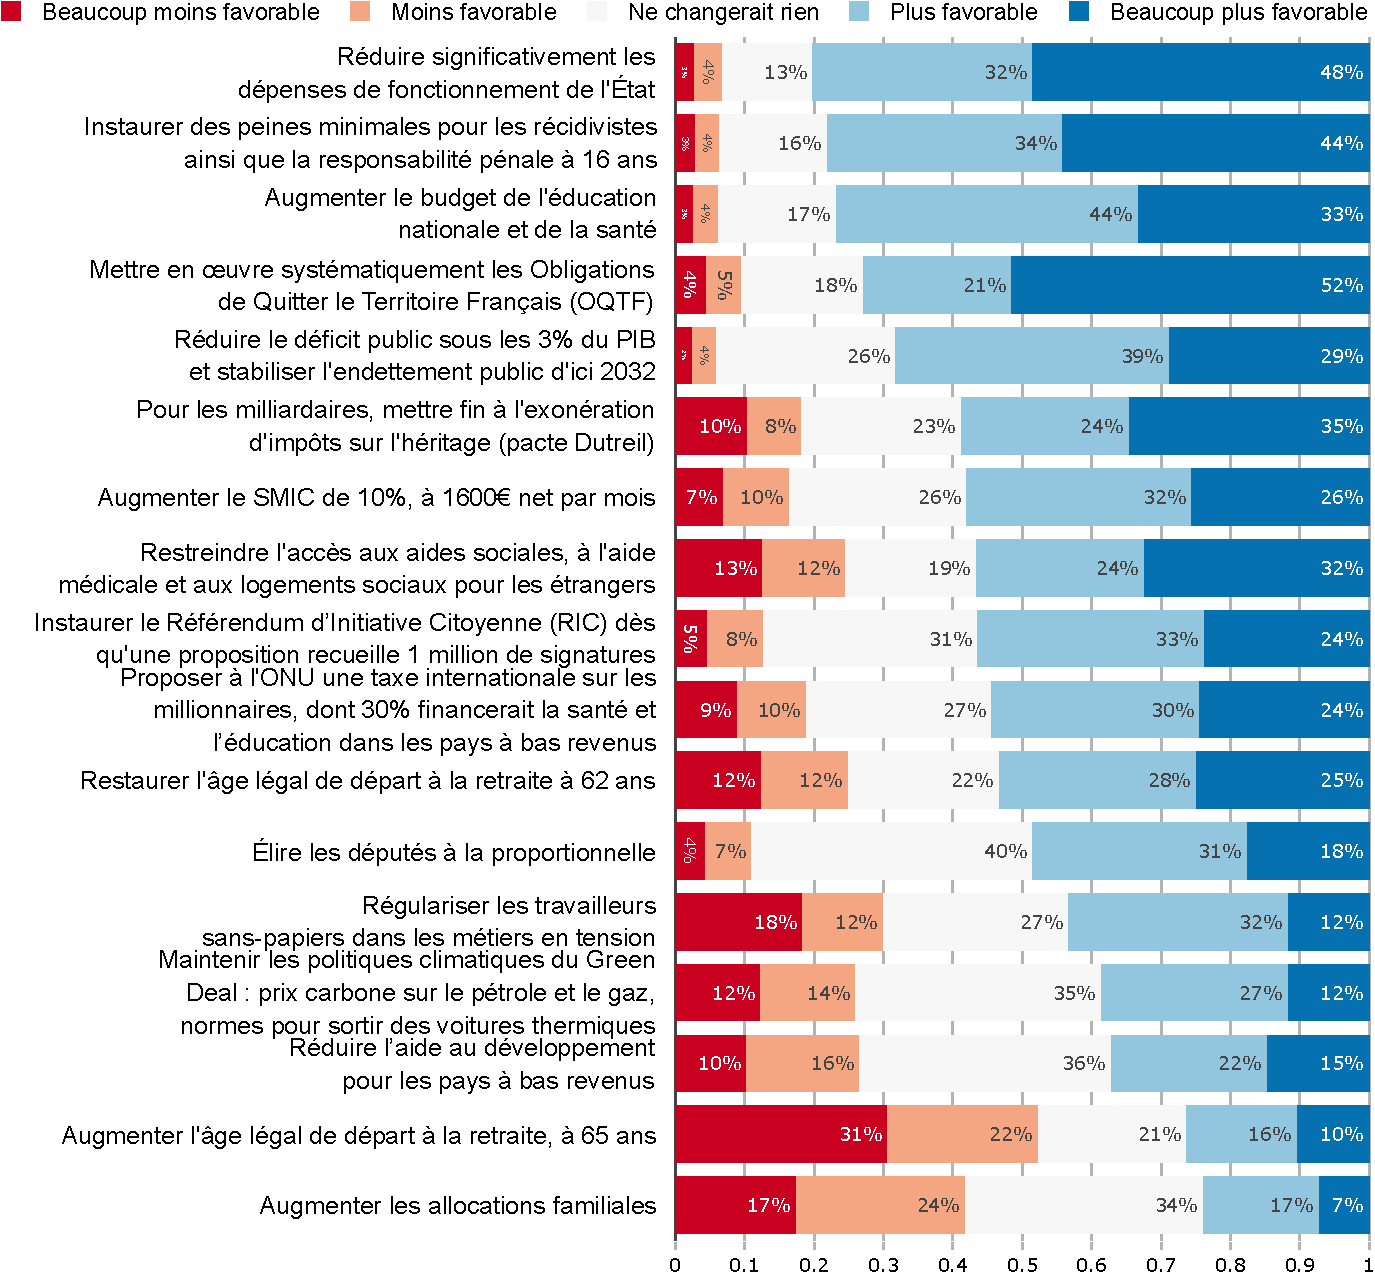
\includegraphics[width=\linewidth]{../figures/effect_program.pdf}
  \caption{Effect of measures on the assessment of a presidential programme.} {\small \textit{For each of the following measures, would its inclusion in a candidate's programme for the 2027 presidential}\\\textit{election make you more or less favorable toward that candidate?}}
  \label{fig:effect_program}
\end{figure}

At the other end of the spectrum, raising the statutory retirement age is rejected by 53\% of the French (and supported by only 26\%).

\subsection{Question \texttt{budget}}

Figure~\ref{fig:budget} presents support for the fiscal measures, ranked by the share of \textit{appropriate} or \textit{desirable} ratings, excluding \textit{Don't know} responses. \blue{The total of measures that a majority finds \textit{appropriate} (or \textit{desirable}) averages 96.9~billion euros in savings (of which 53.2~bn in revenue increases).}
Savings reach 174.8~bn when adding measures that a majority finds \textit{tolerable}, and 31.5~bn when limiting to measures that a majority considers \textit{desirable}.

\begin{figure}[htbp]
  \centering
  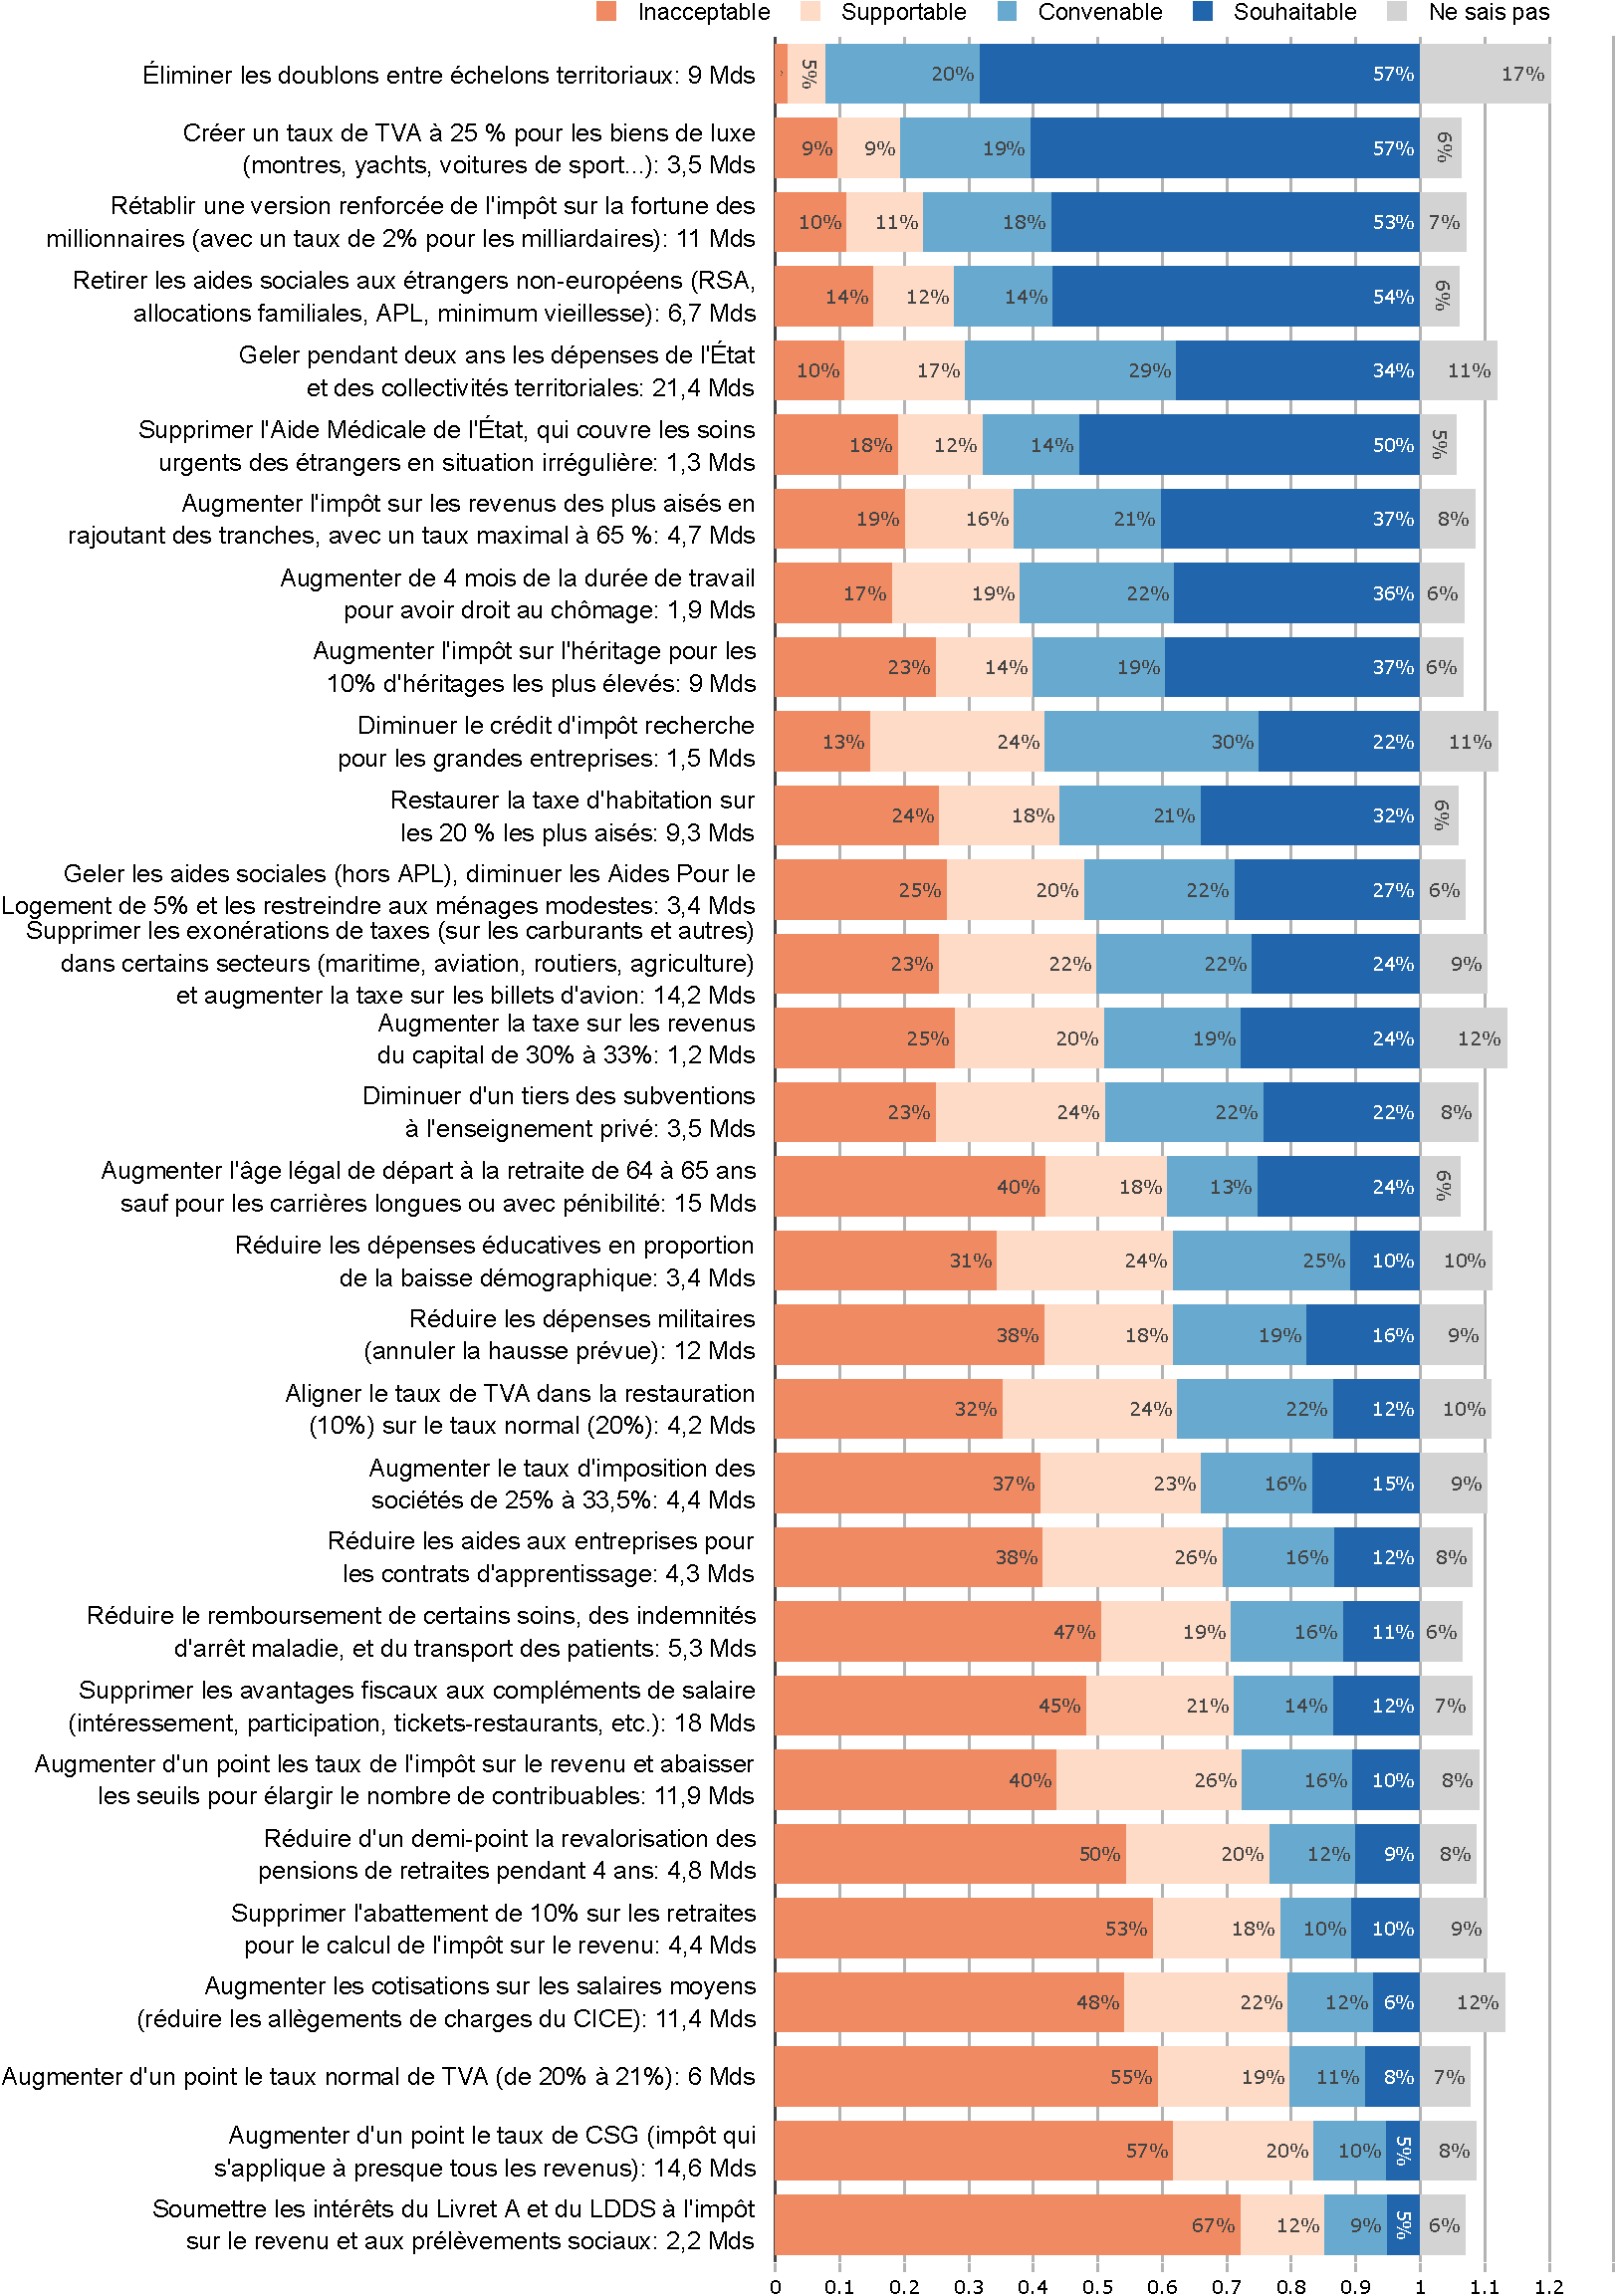
\includegraphics[width=\linewidth]{../figures/budget.pdf}
  \caption{Assessments of fiscal measures.}
  \label{fig:budget}
\end{figure}

\blue{The thirteen measures that a majority finds \textit{appropriate} are primarily taxes on the wealthy (5 measures totaling 37.5~bn), spending freezes or rationalization (2 measures for 30.4~bn), and elimination of welfare benefits for foreigners (2 measures for 8~bn). Raising the statutory retirement age to 65 is \textit{unacceptable} to 40\% of the French, while across-the-board tax hikes (VAT, CSG) or cuts to retirees' living standards are \textit{unacceptable} to a majority.}


%%%%%%%%%%%%%%%%%%%%%%%%%%%%%%%%%%%%%%%%%%%%%%%%%%%%%%%%%%%%%
\section{Determinants of Support}
\label{sec:determinants}
%%%%%%%%%%%%%%%%%%%%%%%%%%%%%%%%%%%%%%%%%%%%%%%%%%%%%%%%%%%%%

I examine here how political attitudes can be predicted from a set of sociodemographic characteristics. For each attitude, I use linear regression to analyze the share of variance explained by each sociodemographic variable. I then average these shares across all attitudes to estimate the predictive power of each sociodemographic characteristic%
\footnote{More precisely, I apply the LMG method to each attitude, meaning that for each attitude I compute the average of the variance decomposition (ANOVA) over all permutations of the sociodemographic variables \citep{lindeman_introduction_1980,gromping_estimators_2007}. The 47 political attitudes studied include each \texttt{budget} variable (recoded between $-1$ and 2) and each \texttt{programme} variable (from $-2$ to 2), as well as two additional variables: the sum of savings implied by measures rated \textit{appropriate} by a respondent, and similarly for measures rated \textit{desirable}. The sociodemographic variables used are: political bloc (grouping of actual or hypothetical vote into three political families), indicators for gender, age, income level, educational attainment, urbanity, region, wealth, employment status, abstention in the European elections, household size and number of children under 14 in the household. Other variables or variable interactions were not retained as their predictive power proved too weak.}.

Sociodemographic characteristics explain 13\% of the variance, a standard figure for political attitudes. This figure can be interpreted through a simple example: it corresponds to the case where one has a 50\% chance of correctly predicting an attitude when nothing is known about the person, and a 68\% chance when their characteristics are known\footnote{In that case, the characteristics yield 36\% additional correct predictions. This means the characteristics explain 36\% of the standard deviation, i.e., a share $0.36^2=0.13$ of the variance.}. For instance, this is the case when 50\% of people support a measure, 68\% of women support it vs. 32\% of men, and gender is the only variable predicting support.

Alone, \blue{party affinity explains 7\% of the variance in attitudes when defined by political bloc (Left, Centre-right/Right or Far right)} and 9\% when defined by political party. Sociodemographic characteristics excluding vote explain 8\% of the variance. The sum of these two values exceeds 13\% because vote is partly explained by other sociodemographic characteristics. When analyzing the \textit{additional} variance explained by each characteristic (i.e., net of variance already explained by other variables), political bloc explains 6\% of the variance, age 1.5\%, wealth 1.3\%, and other variables (gender, income level, educational attainment, municipality size\dots)
less than 1\% (Figure~\ref{fig:lmg})\footnote{Similarly, regressing each attitude on all sociodemographic characteristics, political bloc has at least one significant coefficient in 86\% of regressions, age in 53\%, gender 47\%, wealth 39\%, income level 29\%, and less for other variables.}.

\blue{In other words, political attitudes vary greatly from one individual to another, even within the social groups that typically serve as interpretive frameworks for political disagreements.}
Figures~\ref{fig:notes_groupes_budget} and~\ref{fig:notes_groupes_effect_program} present the average attitudes of respondents from each political bloc regarding \texttt{budget} and \texttt{programme} measures. Typically, on such charts, the horizontal bars would represent confidence intervals for the mean. With our data, such intervals would have been short, and would have allowed us to observe significant gaps between group means. Here, however, I chose instead to convey within-group variability: the horizontal bars represent the mean deviation from the bloc average among individuals on either side of that mean\footnote{The mean deviation from the mean is computed separately for observations above vs. below the mean.}. The bars are thus a way of visualizing the range of differences within each political bloc, and they reveal that attitudes are often as variable within a political bloc as within the population as a whole.

\begin{figure}[htbp]
  \centering
  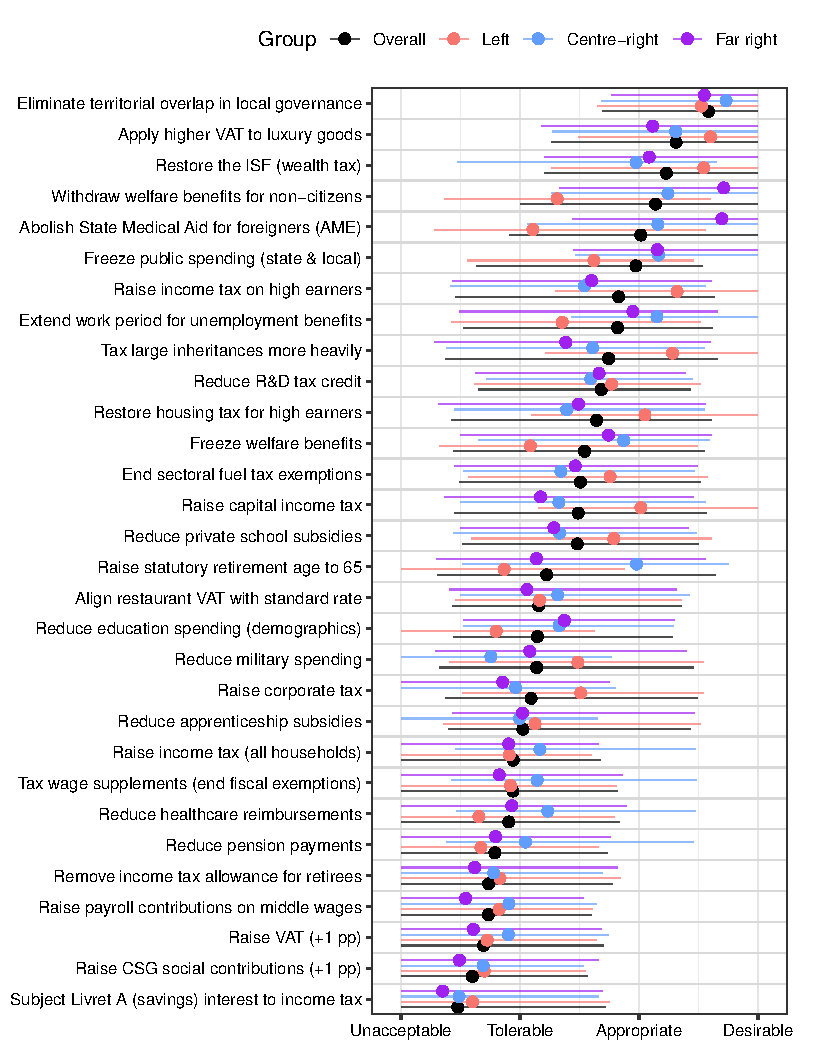
\includegraphics[width=\linewidth]{../figures/notes_groupes_budget_en.pdf}
  \caption{Average assessment of fiscal measures, by political bloc. \\
  {\footnotesize Each lateral bar represents the mean deviation from the bloc average among assessments on the same side of the mean.}}
  \label{fig:notes_groupes_budget}
\end{figure}

\begin{figure}[htbp]
  \centering
  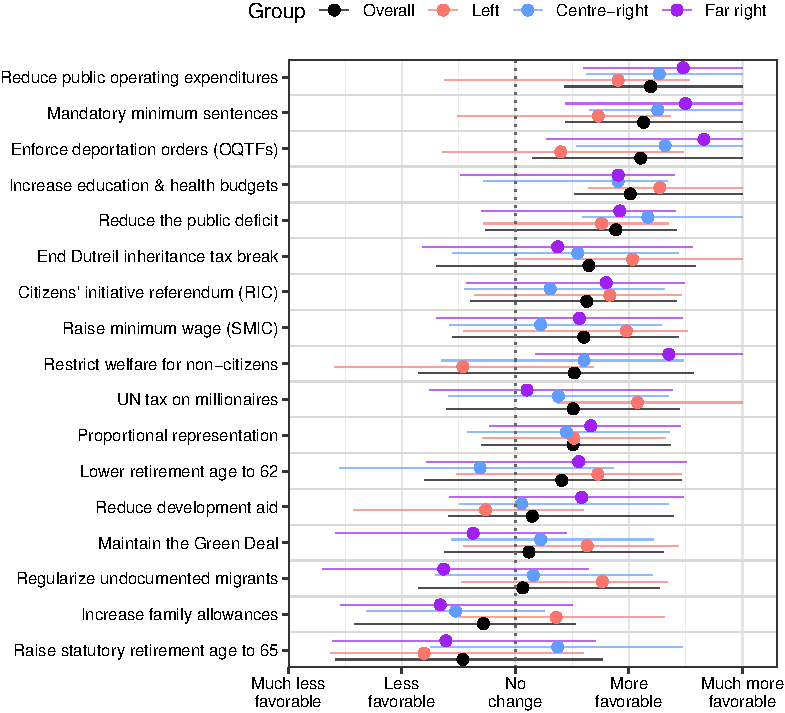
\includegraphics[width=\linewidth]{../figures/notes_groupes_effect_program_en.pdf}
  \caption{Average assessment of programmatic measures, by political bloc. \\
  {\footnotesize Each lateral bar represents the mean deviation from the bloc average among assessments on the same side of the mean.}}
  \label{fig:notes_groupes_effect_program}
\end{figure}

\textbf{What distinguishes the left.} \blue{The sharpest divide between the left and the rest of the electorate concerns nativist measures (withdrawal of benefits for foreigners, elimination of State Medical Aid -- AME).} To a lesser extent, the left more strongly supports taxing the wealthy (inheritance taxes, income tax on high earners).

\textbf{What distinguishes the centre-right.} \blue{Centre-right/right voters are distinguished primarily by their support for raising the statutory retirement age to 65.}

\textbf{What distinguishes the far right.} Far-right voters are generally close to those of the centre-right/right, but beyond the pension question, they stand apart by being more unanimous in favor of restricting welfare benefits for foreigners and relatively opposed to the Green Deal.


%%%%%%%%%%%%%%%%%%%%%%%%%%%%%%%%%%%%%%%%%%%%%%%%%%%%%%%%%%%%%
\section{Distances Between Electoral Groups}
\label{sec:ecarts}
%%%%%%%%%%%%%%%%%%%%%%%%%%%%%%%%%%%%%%%%%%%%%%%%%%%%%%%%%%%%%

To study disparities between electoral groups, I first define the distance between each pair of respondents as the mean of the absolute differences in their ratings on the \texttt{budget} and \texttt{programme} questions\footnote{These questions are recoded from $-1$ to 2 and from $-2$ to 2, respectively. The mean rating is imputed in the case of a \textit{Don't know} response to a \texttt{budget} variable.}.
\blue{The average distance between respondents is 1.16, slightly more than one scale point per response.} Figure~\ref{fig:distance_matrix_pairwise} presents the distances between (respondents from) electoral groups, expressed as the percentage deviation from the average distance between all respondents.
\blue{The greatest distance is observed between LR and LFI voters, at 1.38 (+18.5\% relative to the mean), while the smallest is observed within PS voters, at 1.07 ($-$7.8\%).}

It is instructive to compare inter-individual distance with ``inter-group'' distance, defined as the mean of the absolute differences between two groups' average ratings. The greatest inter-group distance is observed between LFI and LR, at 0.81, i.e., $-$31\% relative to the mean inter-individual distance (see Figure~\ref{fig:distance_matrix_means}), which is smaller than the inter-individual distance within PS voters.
Thus, \blue{there is more disparity in individual attitudes within an electoral group than between the average attitudes of any pair of groups.
This phenomenon may explain why most voters do not identify with any party, as no programme fully satisfies them.}

\blue{Despite the large disparities within each group, inter-individual distances between voters of different parties allow us to reconstruct the political spectrum: (1) PS and Les Écologistes voters are slightly closer to LFI than to the centre-right; (2) centre-right voters are closer to LR than to PS or LÉ; and (3) LR voters are slightly closer to the centre-right than to the far right. Thus, the tripartite structure of Left, Centre-right/Right and Far right emerges naturally from individual preferences. Interestingly, RN voters' attitudes are the closest to those of the electorate as a whole, while LFI voters are the most distant.} These observations are robust to alternative definitions of distance%
\footnote{When distance is defined using the 15 most polarizing attitudes (those with the greatest variance), all observations are confirmed. Only one observation fails when inter-group distance is used: the coalition closest to the electorate as a whole is then the one combining the left and the far right. Similarly, one observation fails when \texttt{programme} variables are recoded between $-1$ and $1$ rather than between $-2$ and $2$ (ignoring the intensity of ratings): LR voters are then closer to the far right than to the centre-right.}.

\begin{figure}[htbp]
  \centering
  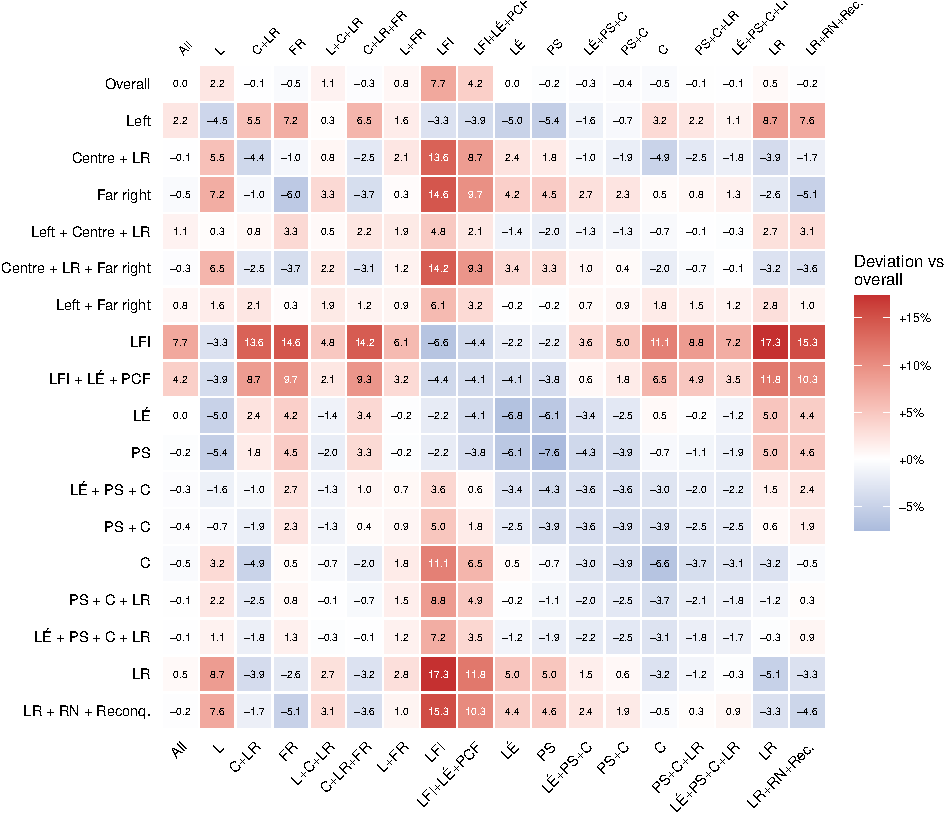
\includegraphics[width=\linewidth]{../figures/distance_matrix_pairwise_en.pdf}
  \caption{Average distances between (and within) electoral groups.}
  {\footnotesize Average inter-individual distance on \texttt{budget} and \texttt{programme} questions, expressed as a percentage deviation from the mean distance within the full sample.}
  \label{fig:distance_matrix_pairwise}
\end{figure}


%%%%%%%%%%%%%%%%%%%%%%%%%%%%%%%%%%%%%%%%%%%%%%%%%%%%%%%%%%%%%
\section{Joint-Majority Policy Packages}
\label{sec:paquets}
%%%%%%%%%%%%%%%%%%%%%%%%%%%%%%%%%%%%%%%%%%%%%%%%%%%%%%%%%%%%%

I search here for policy packages such that the same majority of citizens simultaneously finds each measure in the package acceptable.
In particular, \blue{I identify the \textit{largest} acceptable package, i.e., the package yielding the greatest savings such that a majority of respondents finds none of its measures \textit{unacceptable}}. I carry out this search for the electorate as a whole, but also for voters of each political bloc, each party, and several party coalitions.
Figure~\ref{fig:coalition_packages_matrix} presents the largest packages accepted by a majority within each political grouping.

\blue{The largest package accepted by a majority of respondents saves 69.6~bn through 6 measures: a two-year public spending freeze and elimination of territorial overlap (30.4~bn), increased taxation of the wealthy through the ISF (wealth tax), property tax and income tax (25~bn), and elimination of sectoral fuel tax exemptions (14.2~bn). This package is supported by 57\% of Left voters and by a majority of a coalition formed by Les Écologistes, the PS and the centre-right, but is not supported by a majority of voters in any other coalition.}

The other coalitions considered yield packages with similar savings, with the exception of the Left (LFI--PCF--LÉ--PS), a majority of which accepts a package of 83.3~bn comprising the above package extended by three further fiscal measures targeting the wealthy. Yet left-wing voters do not accept more measures overall: Figure~\ref{fig:coalition_support_heatmap} shows that the total savings from measures rated \textit{appropriate} is similar across political groups, ranging from 89~bn for the median LFI voter to 101~bn for the median LR voter.

Despite the politics of the ``centrist bloc,'' \blue{32.8~bn in additional taxes on the wealthy appear in the centre-right package. Moreover, despite their proximity to LR voters, the centre-right package contains no measures targeting foreigners. It differs from the Left package through the increase in the retirement age and the maintenance of fuel tax exemptions}.

\begin{figure}[htbp]
  \centering
  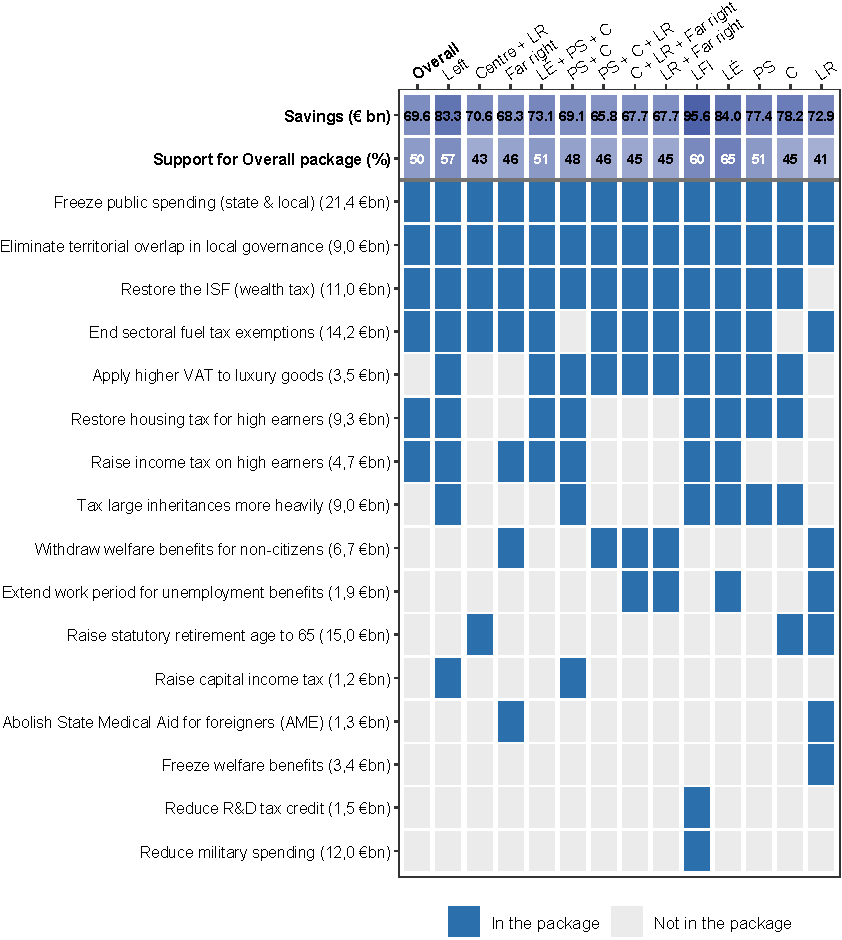
\includegraphics[width=\linewidth]{../figures/coalition_packages_matrix_en.pdf}
  \caption{Largest policy packages accepted by a joint majority, by coalition. \\ {\footnotesize A majority is \textit{joint} if none of the respondents composing it finds any measure in the package \textit{unacceptable}.}}
  \label{fig:coalition_packages_matrix}
\end{figure}

The most widely accepted package achieving at least 90~bn in savings obtains only 34\% joint acceptance. With a more restrictive approach, the largest package of measures that a joint majority finds \textit{appropriate} contains only three measures (elimination of territorial overlap, spending freeze and ISF) for 41.4~bn in savings.

Figure~\ref{fig:coalition_support_heatmap} presents, for each measure, the share of respondents rating it appropriate (or desirable), by electoral coalition. Some measures (elimination of territorial overlap, luxury VAT) receive high support across all groups, while others (withdrawal of benefits for foreigners, pension reform) are highly divisive.


%%%%%%%%%%%%%%%%%%%%%%%%%%%%%%%%%%%%%%%%%%%%%%%%%%%%%%%%%%%%%
\section{Typologies of Respondents and Measures}
\label{sec:clusters}
%%%%%%%%%%%%%%%%%%%%%%%%%%%%%%%%%%%%%%%%%%%%%%%%%%%%%%%%%%%%%

\subsection{Clustering of Respondents}

While I have so far grouped respondents according to their vote, it is instructive to partition them into distinct profiles based on their attitudes. The resulting partition depends on the number $k$ of profiles and the attitudes considered\footnote{I use the $k$-means clustering algorithm for this exercise.}. Whereas Table~\ref{tab:cluster_comparison} presents various clusterings obtained by varying these configurations, one particular clustering draws my attention: the one based on attitudes toward \texttt{budget} measures. This clustering is interesting because it illustrates how the profile that emerges as ``progressive'' could command a majority, even though the left represents only a third of voters. By contrast,
clusterings that incorporate the \texttt{programme} question yield \textit{progressive} profiles that remain a minority.

\blue{The partition presented uses \texttt{budget} and creates three profiles}\footnote{I choose $k$=3 profiles because in our case this maximizes the \textit{silhouette coefficient}, i.e., the relevance of the partition.}, which can be named as follows:

\begin{enumerate}
  \item \blue{\textbf{The conservatives} (48\% of respondents)}: as reported in Table~\ref{tab:cluster_vote}, this profile brings together a majority of right-wing voters (from the centre-right to the far right). However, unlike right-wing voters, support for measures taxing the wealthy is generally minority among the \textit{conservatives} (with exceptions: a majority of \textit{conservatives} supports the ISF, see Figure~\ref{fig:clusters_combined_polarises}).
  \item \blue{\textbf{The progressives} (31\%)}~: the majority profile among left-wing voters.
  Unsurprisingly, a majority of \textit{progressives} supports taxing the wealthy or maintaining the welfare state, and opposes across-the-board taxes or nativist measures.
  \item \blue{\textbf{The deficit hawks} (21\%): this profile is distinguished by majority support for most fiscal consolidation measures, including nativist measures, welfare state restrictions, and (unpopular) across-the-board taxes.} This profile does not correspond to any party and is barely over-represented among centre-right or right-wing voters. \blue{The \textit{deficit hawks} stand out by the total of measures they support:
  on average 146~bn in measures rated \textit{appropriate} or \textit{desirable}, compared to 93~bn for all respondents.}
\end{enumerate}

\begin{table}[htbp]
  \centering
  \caption{Respondent profiles by political bloc in \texttt{budget} clusterings.}
  \label{tab:cluster_vote}
  \begin{tabular}{clccccc}
\toprule
& & & \multicolumn{4}{c}{Part du profil dans le bloc politique (\%)} \\
\cmidrule(lr){4-7}
$k$ & \makecell[l]{Description\\du profil} & \makecell{Taille\\du profil\\(\%)} & \makecell{Gauche\\\quad\\(28\,\%)}  & \makecell{Centre-droit/\\Droite\\(25\,\%)}  & \makecell{Extrême-\\droite\\(30\,\%)}  & \makecell{Non-réponse/\\Autre\\(17\,\%)} 
 \\
\midrule
2 & \cellcolor{mgt!15}Sociaux & \cellcolor{mgt!15}54 & \cellcolor{mgt!15}83 & \cellcolor{mgt!15}39 & \cellcolor{mgt!15}38 & \cellcolor{mgt!15}56
 \\
 & \cellcolor{cdroite!15}Conservateurs & \cellcolor{cdroite!15}46 & \cellcolor{cdroite!15}17 & \cellcolor{cdroite!15}61 & \cellcolor{cdroite!15}62 & \cellcolor{cdroite!15}44
 \\
\midrule
3 & \cellcolor{cleft!15}Progressistes & \cellcolor{cleft!15}31 & \cellcolor{cleft!15}62 & \cellcolor{cleft!15}17 & \cellcolor{cleft!15}13 & \cellcolor{cleft!15}33
 \\
 & \cellcolor{cfrug!15}Frugaux & \cellcolor{cfrug!15}21 & \cellcolor{cfrug!15}22 & \cellcolor{cfrug!15}28 & \cellcolor{cfrug!15}19 & \cellcolor{cfrug!15}15
 \\
 & \cellcolor{cdroite!15}Conservateurs & \cellcolor{cdroite!15}48 & \cellcolor{cdroite!15}16 & \cellcolor{cdroite!15}55 & \cellcolor{cdroite!15}68 & \cellcolor{cdroite!15}52
 \\
\midrule
4 & \cellcolor{cleft!15}Progressistes & \cellcolor{cleft!15}21 & \cellcolor{cleft!15}55 & \cellcolor{cleft!15}9 & \cellcolor{cleft!15}3 & \cellcolor{cleft!15}15
 \\
 & \cellcolor{cfrug!15}Frugaux & \cellcolor{cfrug!15}18 & \cellcolor{cfrug!15}20 & \cellcolor{cfrug!15}25 & \cellcolor{cfrug!15}14 & \cellcolor{cfrug!15}12
 \\
 & \cellcolor{ccdroit!15}Libéraux-nativistes & \cellcolor{ccdroit!15}24 & \cellcolor{ccdroit!15}8 & \cellcolor{ccdroit!15}35 & \cellcolor{ccdroit!15}34 & \cellcolor{ccdroit!15}21
 \\
 & \cellcolor{ced!15}Sociaux-nativistes & \cellcolor{ced!15}36 & \cellcolor{ced!15}17 & \cellcolor{ced!15}31 & \cellcolor{ced!15}50 & \cellcolor{ced!15}53
 \\
\bottomrule
\end{tabular}

\end{table}

This automatic tripartition yields profiles somewhat different from the usual political blocs, in particular the \textit{deficit hawks}. When the exercise is repeated with four profiles rather than three, the \textit{deficit hawks} profile reappears almost intact (18\% of respondents), while \blue{the \textit{conservatives} split into two groups: 24\% of \textit{liberal-nativists} who are largely opposed to taxes on the wealthy, and 36\% of \textit{social-nativists} who are mostly in favor of them}. Note that the \textit{social-nativists}, while largely drawn from \textit{conservatives}, also include about a third of the \textit{progressives}, essentially those who support nativist measures. Although the \textit{social-nativists} broadly overlap with far-right voters,
they are more favorable to taxes on the wealthy than those voters; their attitudes thus do not correspond to any existing partisan offer.

\blue{It is instructive to reproduce the exercise with a partition into two profiles rather than three. One then observes a profile of 46\% of relatively unchanged \textit{conservatives}, and a coalition of the \textit{deficit hawks} and the \textit{progressives} within a majority profile I term the \textit{social coalition}. This electoral partition could potentially emerge at the 2027 presidential election in the event of a second round between a candidate who unites the conservative camp and another who succeeds in simultaneously addressing the main concerns of the \textit{progressives} (inequality) and the \textit{deficit hawks} (the deficit).}

In such a scenario, the left would ally with fiscally hawkish nativists around issues of taxing the wealthy and deficit reduction. \blue{Conversely, if the political game puts migration front and center and the right-wing candidate appears more credible on deficit reduction, the electorate would partition differently and would likely hand victory to the \textit{conservatives}.} This is the scenario that occurs when \texttt{programme} measures are used to identify the partition (see Table~\ref{tab:cluster_comparison}).


\subsection{Clustering of Measures}

Just as respondents have been partitioned according to their attitudes, one can here partition the \texttt{budget} measures according to the respondents who support them\footnote{This time, the different configurations yield partitions that are fairly close to one another. The partition into two sets separates popular from unpopular measures (except when performed on \texttt{programme} measures alone, where the separation is left/right). The three-way partition of all measures is almost the union of the partitions performed separately on \texttt{budget} or \texttt{programme} measures (except for the reduction of development aid, which is \textit{right-wing} in the \texttt{programme} partition but \textit{unpopular} when all measures are considered). Partitions into four sets cause the left-leaning measures to split between those majority-supported in each bloc vs. only on the left.}.
As shown in Table~\ref{tab:cluster_measures_budget3}, \blue{the three sets of measures identified correspond fairly well to the three respondent profiles studied above}. We distinguish:

\begin{enumerate}
  \item 15 \textbf{unpopular measures} (total savings: 122~bn): across-the-board taxes; retirement at 65; reduced military spending, apprenticeship subsidies or healthcare reimbursements\dots{} These measures are rejected by most respondents, except among the \textit{deficit hawks}.
  \item 9 \textbf{left-leaning measures} (58~bn): taxes on the wealthy, elimination of sectoral fuel tax exemptions\dots{} These measures are on average supported by a majority in each political bloc, very popular among the left as well as among \textit{progressives} and the \textit{deficit hawks}, but minority among \textit{conservatives}.
  \item 6 \textbf{right-leaning measures} (44~bn): rationalization or freeze of public spending or welfare benefits, nativist measures\dots{} These measures are majority-supported in each political bloc, very popular on the right as well as among \textit{conservatives} and the \textit{deficit hawks}, but minority among \textit{progressives}.
\end{enumerate}

\blue{While measures divide largely along the left/right divide,
the composition of voters supporting each set of measures in fact varies little from one set to another}\footnote{Coding political bloc between $-$0.1 (Left) and 1 (Far right), the average political bloc varies from $-$0.1 for respondents supporting left-leaning measures to 0.2 for those supporting right-leaning measures (see Figure~\ref{tab:cluster_measures_budget3}).}.

\begin{table}[htbp]
  \centering\footnotesize\setlength{\tabcolsep}{4pt}\caption{Support for \texttt{budget} measure sets identified by clustering ($k$=3).}
  \noindent\makebox[\textwidth][c]{%
\begin{tabular}{lcccccccc}
\toprule
& & \multicolumn{4}{c}{Soutien moyen par bloc politique (\%)} & \multicolumn{3}{c}{Soutien moyen par profil (\%)} \\
\cmidrule(lr){3-6}\cmidrule(lr){7-9}
\makecell[l]{Ensemble de mesures\\(nombre; \textit{économies})} & \makecell{Bloc\\pol.\\moyen} & \makecell{Gauche} & \makecell{Centre-\\droit/\\Droite} & \makecell{Extr.-\\droite} & \makecell{Non-\\rép./\\Autre} & \makecell{Progres-\\sistes} & \makecell{Frugaux} & \makecell{Conser-\\vateurs}
 \\
\midrule
\textbf{De gauche} (9; \textit{57,9~Mds}) & $-$0,1 & 72 & 53 & 54 & 62 & 76 & 76 & 41
 \\
\textbf{Impopulaires} (15; \textit{121,9~Mds}) & \phantom{$-$}0,0 & 28 & 32 & 27 & 24 & 19 & 57 & 20
 \\
\textbf{De droite} (6; \textit{43,7~Mds}) & \phantom{$-$}0,2 & 51 & 76 & 80 & 70 & 47 & 83 & 79
 \\
\bottomrule
\end{tabular}}

  \par\smallskip
  {\footnotesize \textit{Note:} Support is defined as the share of \textit{appropriate} or \textit{desirable} ratings within the considered respondent groups. \textit{Political bloc} codes actual or hypothetical vote between $-$1 (Left) and 1 (Far right). The right-hand columns report average support by political bloc and by profile identified by clustering respondents using \texttt{budget} ratings ($k=3$).}
  \label{tab:cluster_measures_budget3}
\end{table}

To complement this analysis, Figure~\ref{fig:budget_correlations} presents the correlations in support between measures. There is a strong correlation between nativist measures,
a positive correlation among the various taxes on the wealthy, and a negative correlation between welfare state restriction measures and those taxing the wealthy.


%%%%%%%%%%%%%%%%%%%%%%%%%%%%%%%%%%%%%%%%%%%%%%%%%%%%%%%%%%%%%
\section{Comparison with La Plateforme Progressiste}
\label{sec:progressistes}
%%%%%%%%%%%%%%%%%%%%%%%%%%%%%%%%%%%%%%%%%%%%%%%%%%%%%%%%%%%%%

\blue{La Plateforme Progressiste is an initiative aimed at establishing the programme of a ``progressive arc [ranging] from those who say no to a project with Les Républicains for 2027 to those who say no to La France Insoumise''}\footnote{Source: interview with Pascal Canfin in \href{https://www.lemonde.fr/politique/article/2025/07/01/pascal-canfin-personne-parmi-les-progressistes-ne-pourra-gagner-seul-l-election-presidentielle_6617180_823448.html}{Le Monde}.}. During an online consensus conference in late 2025, approximately 150 supporters voted on various fiscal savings measures. The \href{https://laplateformeprogressiste.org/wp-content/uploads/2025/12/20251210_Resultats-par-mesure-1.pdf}{measures supported} by a majority of respondents total 99.9~bn in savings, a figure close to the average of 96.9~bn in \textit{appropriate} measures in our sample. Measures supported by a majority of the Progressive Platform include rationalization of public spending, elimination of sectoral fuel tax exemptions, taxation of the wealthy, and savings on (particularly affluent) retirees. \blue{Participants in this exercise have fiscal preferences close to those of PS voters}: unlike centre-right voters, they are mostly opposed to raising the statutory retirement age and mostly in favor of environmental taxes. Unlike the majority of French citizens, Progressive Platform supporters are broadly opposed to measures targeting foreigners, and more favorable to institutionally endorsed measures that were probably justified during the consensus conference, such as reducing apprenticeship subsidies or eliminating the tax allowance for retirees' professional expenses.
This comparison illustrates the role that information and deliberation can play in shaping attitudes, even if it could also reflect a selection bias among conference participants.


%%%%%%%%%%%%%%%%%%%%%%%%%%%%%%%%%%%%%%%%%%%%%%%%%%%%%%%%%%%%%
\section{Discussion}
\label{sec:conclusion}
%%%%%%%%%%%%%%%%%%%%%%%%%%%%%%%%%%%%%%%%%%%%%%%%%%%%%%%%%%%%%

This survey reveals majority support for measures spanning the political spectrum: the ISF (wealth tax), rationalization of public spending, increased education and health budgets, systematic enforcement of deportation orders (OQTFs), deficit reduction, etc. Similarly, a majority rejects measures from both left and right: raising the retirement age, increasing family allowances, reducing military spending, etc.

Thus, while attitudes are shaped by political mobilization and identity (as shown by the rejection of raising the retirement age, which is consensual in a country like Denmark), voters are not perfectly aligned with the parties for which they vote. For example, despite some candidates' opposition, \blue{restoring the ISF or introducing citizens' initiative referendums (RIC) are supported by a majority of voters in every party}\footnote{Here, \textit{majority support} means an \textit{appropriate} or \textit{desirable} rating for the ISF, and a majority of \textit{favorable} responses excluding \textit{indifferent} for the RIC.}. These results suggest that policy outcomes depend on institutions, and that a direct democracy (even partial, through the RIC) would implement both nativist and redistributive measures, from otherwise opposing camps.

To understand what budget a majority coalition could implement, the question is not merely to juxtapose the 97~bn in appropriate measures for different majorities, but to find a package of measures jointly accepted by the same majority. \blue{The majority package allowing the greatest savings (70~bn) combines 30~bn in public spending restraint, 25~bn in taxes on the wealthy, and 14~bn in environmental taxes}. This package is supported by a majority of voters in each left-wing party, and by a majority of a coalition of green, socialist and centrist voters\footnote{The vote considered is that of the 2024 European elections.}. While the largest majority package among left-wing voters alone extends this package with an additional 13~bn in taxes on the wealthy, those of far-right voters or of the centre and right remain at a similar savings level, replacing 10 to 15~bn in taxes on the wealthy with withdrawal of welfare benefits for foreigners or the retirement-at-65 measure, respectively.

Note that even when popular, some measures would be difficult to implement with the expected results. For instance, a two-year freeze on public spending (in volume terms, excluding inflation) is merely a framework and would require further (a priori unpopular) measures to offset the structural spending increase (driven notably by demographic ageing and the military programming law). Some measures raise issues of constitutional and international law compliance: mandatory minimum sentences conflict with the constitutional principles of individualization of sentences and proportionality; the Constitutional Council has struck down the limitation of the property tax to high earners; it is uncertain whether it would validate a wealth tax rate above 1\% (though adoption by referendum would bypass constitutional review); EU law prevents the systematic enforcement of OQTFs by requiring individual case assessment and a right of appeal; and the European Court of Human Rights (ECHR) holds that social benefits (such as family allowances and State Medical Aid) meet essential needs and that discrimination based on nationality would be unjustified. Finally, savings estimates from certain measures such as the elimination of territorial overlap (9~bn) or the luxury VAT (3.5~bn) may have been overstated.

Deficit reduction promises to be as difficult as it is necessary.
Certainly, economists such as \cite{geerolf_dette_2021} remind us that the deficit should not be fetishized (and that the composition of the budget matters more), that a high deficit can be justified to absorb a shock or fund forward-looking expenditure (especially if temporary), and that any level of debt is sustainable as long as growth exceeds the interest rate on outstanding debt. But precisely, this last condition is not guaranteed; and even when it holds, it is often preferable to reduce indebtedness to avoid rising interest rates \citep{mian_goldilocks_2025}. Moreover, all parties agree on the need to reduce the deficit; disagreement now concerns the desirable magnitude of the reduction. While the survey adopted the CAE's fiscal adjustment target of 90~bn, \cite{delatte_redresser_2025} calculates that debt could be stabilized with an effort of only 43~bn,
by coupling 120~bn in consolidation (half in taxes on the wealthy) with 75~bn in additional spending, which would avoid the recessionary effects of austerity by placing the burden on high-income households, whose propensity to consume is low.
If the author is right to account for the so-called \textit{multiplier} effects of each measure, some of her assumptions are contestable, notably the legal and geopolitical feasibility of a unilateral 25\% tax on multinational profits earned in France (estimated to raise 26~bn).

But whether the target is 43~bn or 90~bn, the effort will be significant. \blue{The next government will face difficult choices; it will have to resolve to either tax the wealthy, or be unpopular, or let public debt spiral out of control -- and doubtless a little of all three at once.}
While the largest majority package resembles a left-wing programme (with redistributive measures and no nativist ones), a majority of the electorate leans rather to the right or far right, motivated by opposition to ``welfare dependency,'' the appeal of growth, or a desire for security.
Thus, \blue{the presidential election will likely be won by the candidate who achieves the best synthesis between redistribution, fiscal credibility and law-and-order firmness}, reconciling diverse aspirations, some of which risk alienating their own camp.

Although \blue{the structuring of the electorate into three blocs (left, centre-right/right, far right) emerges naturally from fiscal preferences} when one analyzes proximity between electoral groups, these blocs are not fixed. While many voters are loyal to their camp, programmatic attitudes are stable and as predictive of voting behavior as political identity \citep{ansolabehere_strength_2008}. As a result, a party risks losing voters if its programme no longer matches their attitudes, and failing to attract new ones if it does not adjust its positioning.

\blue{The left differs from the rest of the electorate through its rejection of nativism. To win, it will likely need to} avoid championing unpopular measures such as creating a climate refugee status or cutting military spending, and instead \blue{insist on sound public finances, arguing that the deficit cannot be reduced without taxing the wealthy}.

\blue{The centre-right and LR are distinguished by their support for raising the retirement age and are out of step with their own voters on wealth taxation}. While advantaged by their position at the center of the political spectrum and by a reputation as a responsible, economically realistic bloc (since their programme prioritizes growth), the centrist bloc will struggle to win on a ``blood, sweat and tears'' promise, as a majority would prefer to tax the wealthy rather than work longer. In this respect, Gabriel Attal's position in favor of a points-based pension system appears more promising than Édouard Philippe's hints at raising the statutory retirement age to 67. Attal's proposal would allow each person to choose their own retirement age, with the pension amount adjusted to ensure fiscal neutrality.

The far right relies on an electoral base with both social and nativist aspirations. Electorally, \blue{the RN would likely make a mistake by not proposing a credible fiscal programme. Indeed, our analysis indicates that the profile that could deliver a majority for the far right consists of \textit{deficit-hawk} voters primarily concerned with deficit reduction}, who could turn to any candidate credible on this issue.

Given the fragmentation of the political spectrum, parties will likely have to accept compromises and form alliances to govern, at the risk of moving their programmes further from their voters. Such maneuvers could contribute to the \blue{widespread dissatisfaction with the political class as a whole}, since parties already bring together heterogeneous voters: \blue{heterogeneity is greater among voters of the same party than between the average attitudes of voters of different parties.}
That said, many French citizens are weary of the current polarization and might actually welcome a coalition that transcends the usual divides.
In any case, the choice of alliances will be particularly agonizing for the PS and the Greens, from the very next Finance Bill onwards, caught between the inadequacy of an alliance with the centre (given the greater proximity of their voters' preferences to LFI's programme) and the rejection of LFI's provocative and peremptory tone by most French citizens, including many of their own voters\footnote{Beyond the survey data, this paragraph draws on individual interviews conducted with a representative sample of 100 French citizens.}.

While hoping to contribute to the quality of public debate, one must acknowledge the limitations of this analysis. To begin with, the importance of deficit reduction for voters may have been overstated, given the focus of the analysis. The necessary conciseness of the survey meant omitting certain domains (foreign policy, the European project\dots{}) and certain proposals (full restoration of the property tax, maximum inheritance limits\dots{}) that may prove decisive. Moreover, the precision of results for subgroups must be tempered by the sample size. Finally, attitudes may evolve during public debate. In this respect, one can only welcome initiatives such as consensus conferences or ``living-room meetings'' that allow citizens to deliberate, confront arguments and refine their views.

To enable voters to make an informed choice, it would also be very useful to import a practice from the Netherlands, where each party presents a programme of specific measures, subsequently evaluated by an independent body. In France, organizations such as the OFCE and the IPP could perform this task of simulating party programmes in terms of debt trajectories, growth, inequality, greenhouse gas emissions and demography.

\bigskip

\clearpage
\bibliographystyle{plainnaturl_clean}
\bibliography{budget}

%%%%%%%%%%%%%%%%%%%%%%%%%%%%%%%%%%%%%%%%%%%%%%%%%%%%%%%%%%%%%
\appendix
\renewcommand{\thefigure}{A\arabic{figure}}
\setcounter{figure}{0}
\renewcommand{\thetable}{A\arabic{table}}
\setcounter{table}{0}

\section{Appendix}


\begin{figure}[htbp]
  \centering
  \begin{subfigure}[b]{0.49\textwidth}
    \centering
    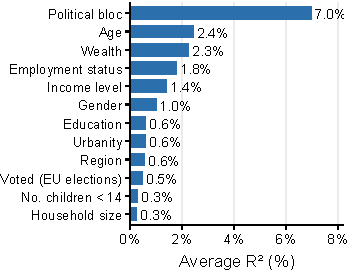
\includegraphics[width=\linewidth]{../figures/r2_iso_attitudes_en.pdf}
    \subcaption{Isolated R\textsuperscript{2} (one regressor at a time).}
    \label{fig:r2_iso_attitudes}
  \end{subfigure}\hfill
  \begin{subfigure}[b]{0.49\textwidth}
    \centering
    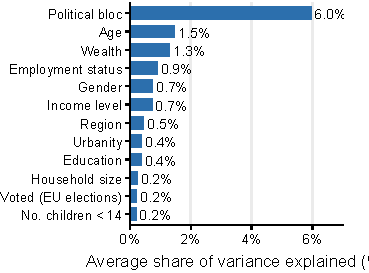
\includegraphics[width=\linewidth]{../figures/lmg_attitudes_en.pdf}
    \subcaption{R\textsuperscript{2} decomposition (joint regression).}
    \label{fig:lmg_attitudes}
  \end{subfigure}
  \caption{Variance in attitudes explained by sociodemographic characteristics. (a) Average R\textsuperscript{2} obtained by regressing each attitude on one characteristic at a time; (b) average share of variance explained by each characteristic in the joint regression (LMG decomposition, total explained variance: 13\%). Averages are computed over the 47 attitude variables (\texttt{budget} and \texttt{programme} measures and the \texttt{sum\_acceptable} and \texttt{sum\_desirable} indices).}
  \label{fig:lmg}
\end{figure}

\begin{figure}[htbp]
  \centering
  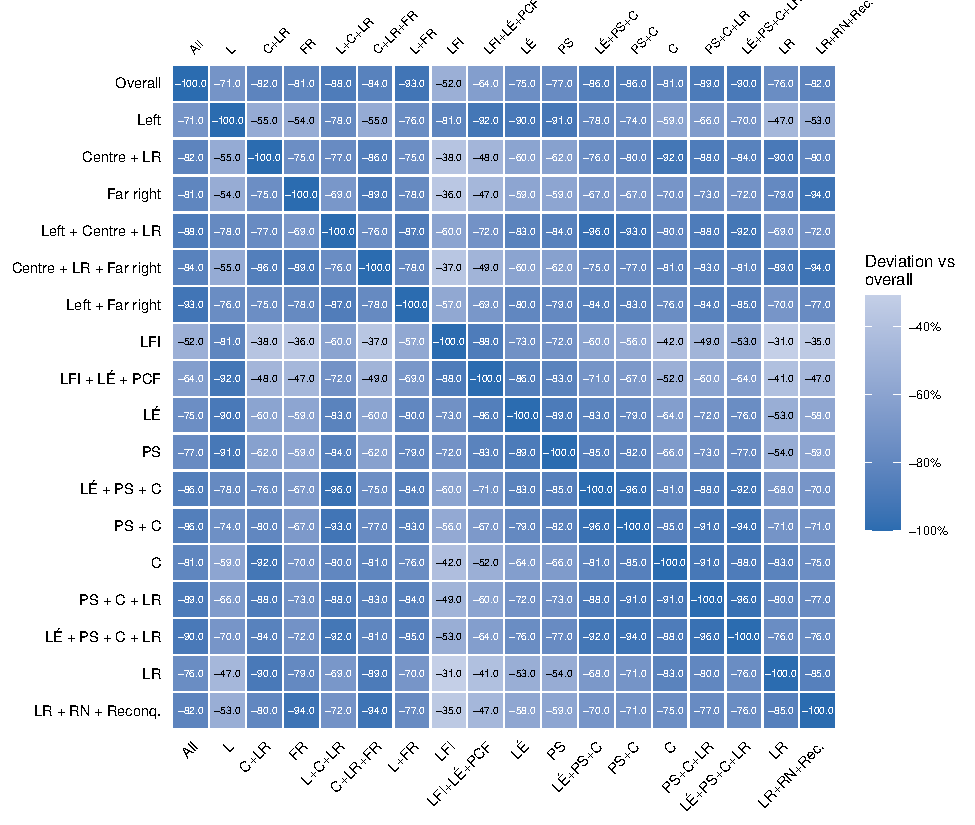
\includegraphics[width=\linewidth]{../figures/distance_matrix_means_en.pdf}
  \caption{Distances between average attitudes for each pair of electoral groups.}
  {\footnotesize Distance between average attitudes of electoral groups on \texttt{budget} and \texttt{programme} questions, expressed as a percentage deviation from the mean inter-individual distance within the full sample.}
  \label{fig:distance_matrix_means}
\end{figure}

\begin{figure}[htbp]
  \centering
  \vspace{-1cm}
  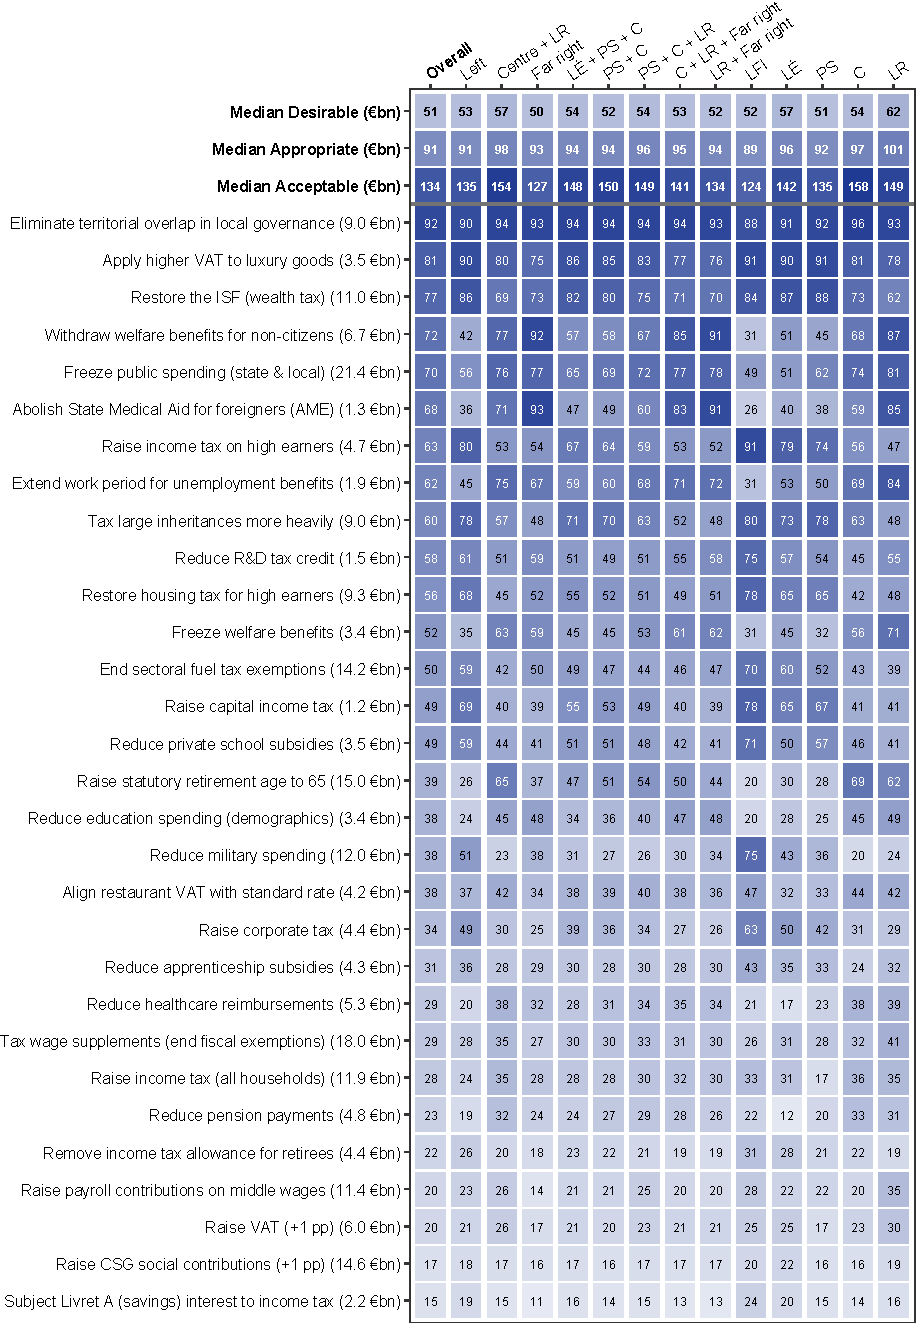
\includegraphics[width=\linewidth]{../figures/coalition_support_heatmap_en.pdf}
  \caption{Share of \textit{appropriate} or \textit{desirable} ratings per measure and per coalition (in \%). The first three rows report the median total savings supported by respondents in each coalition.}
  \label{fig:coalition_support_heatmap}
\end{figure}

\begin{figure}[htbp]
  \centering
  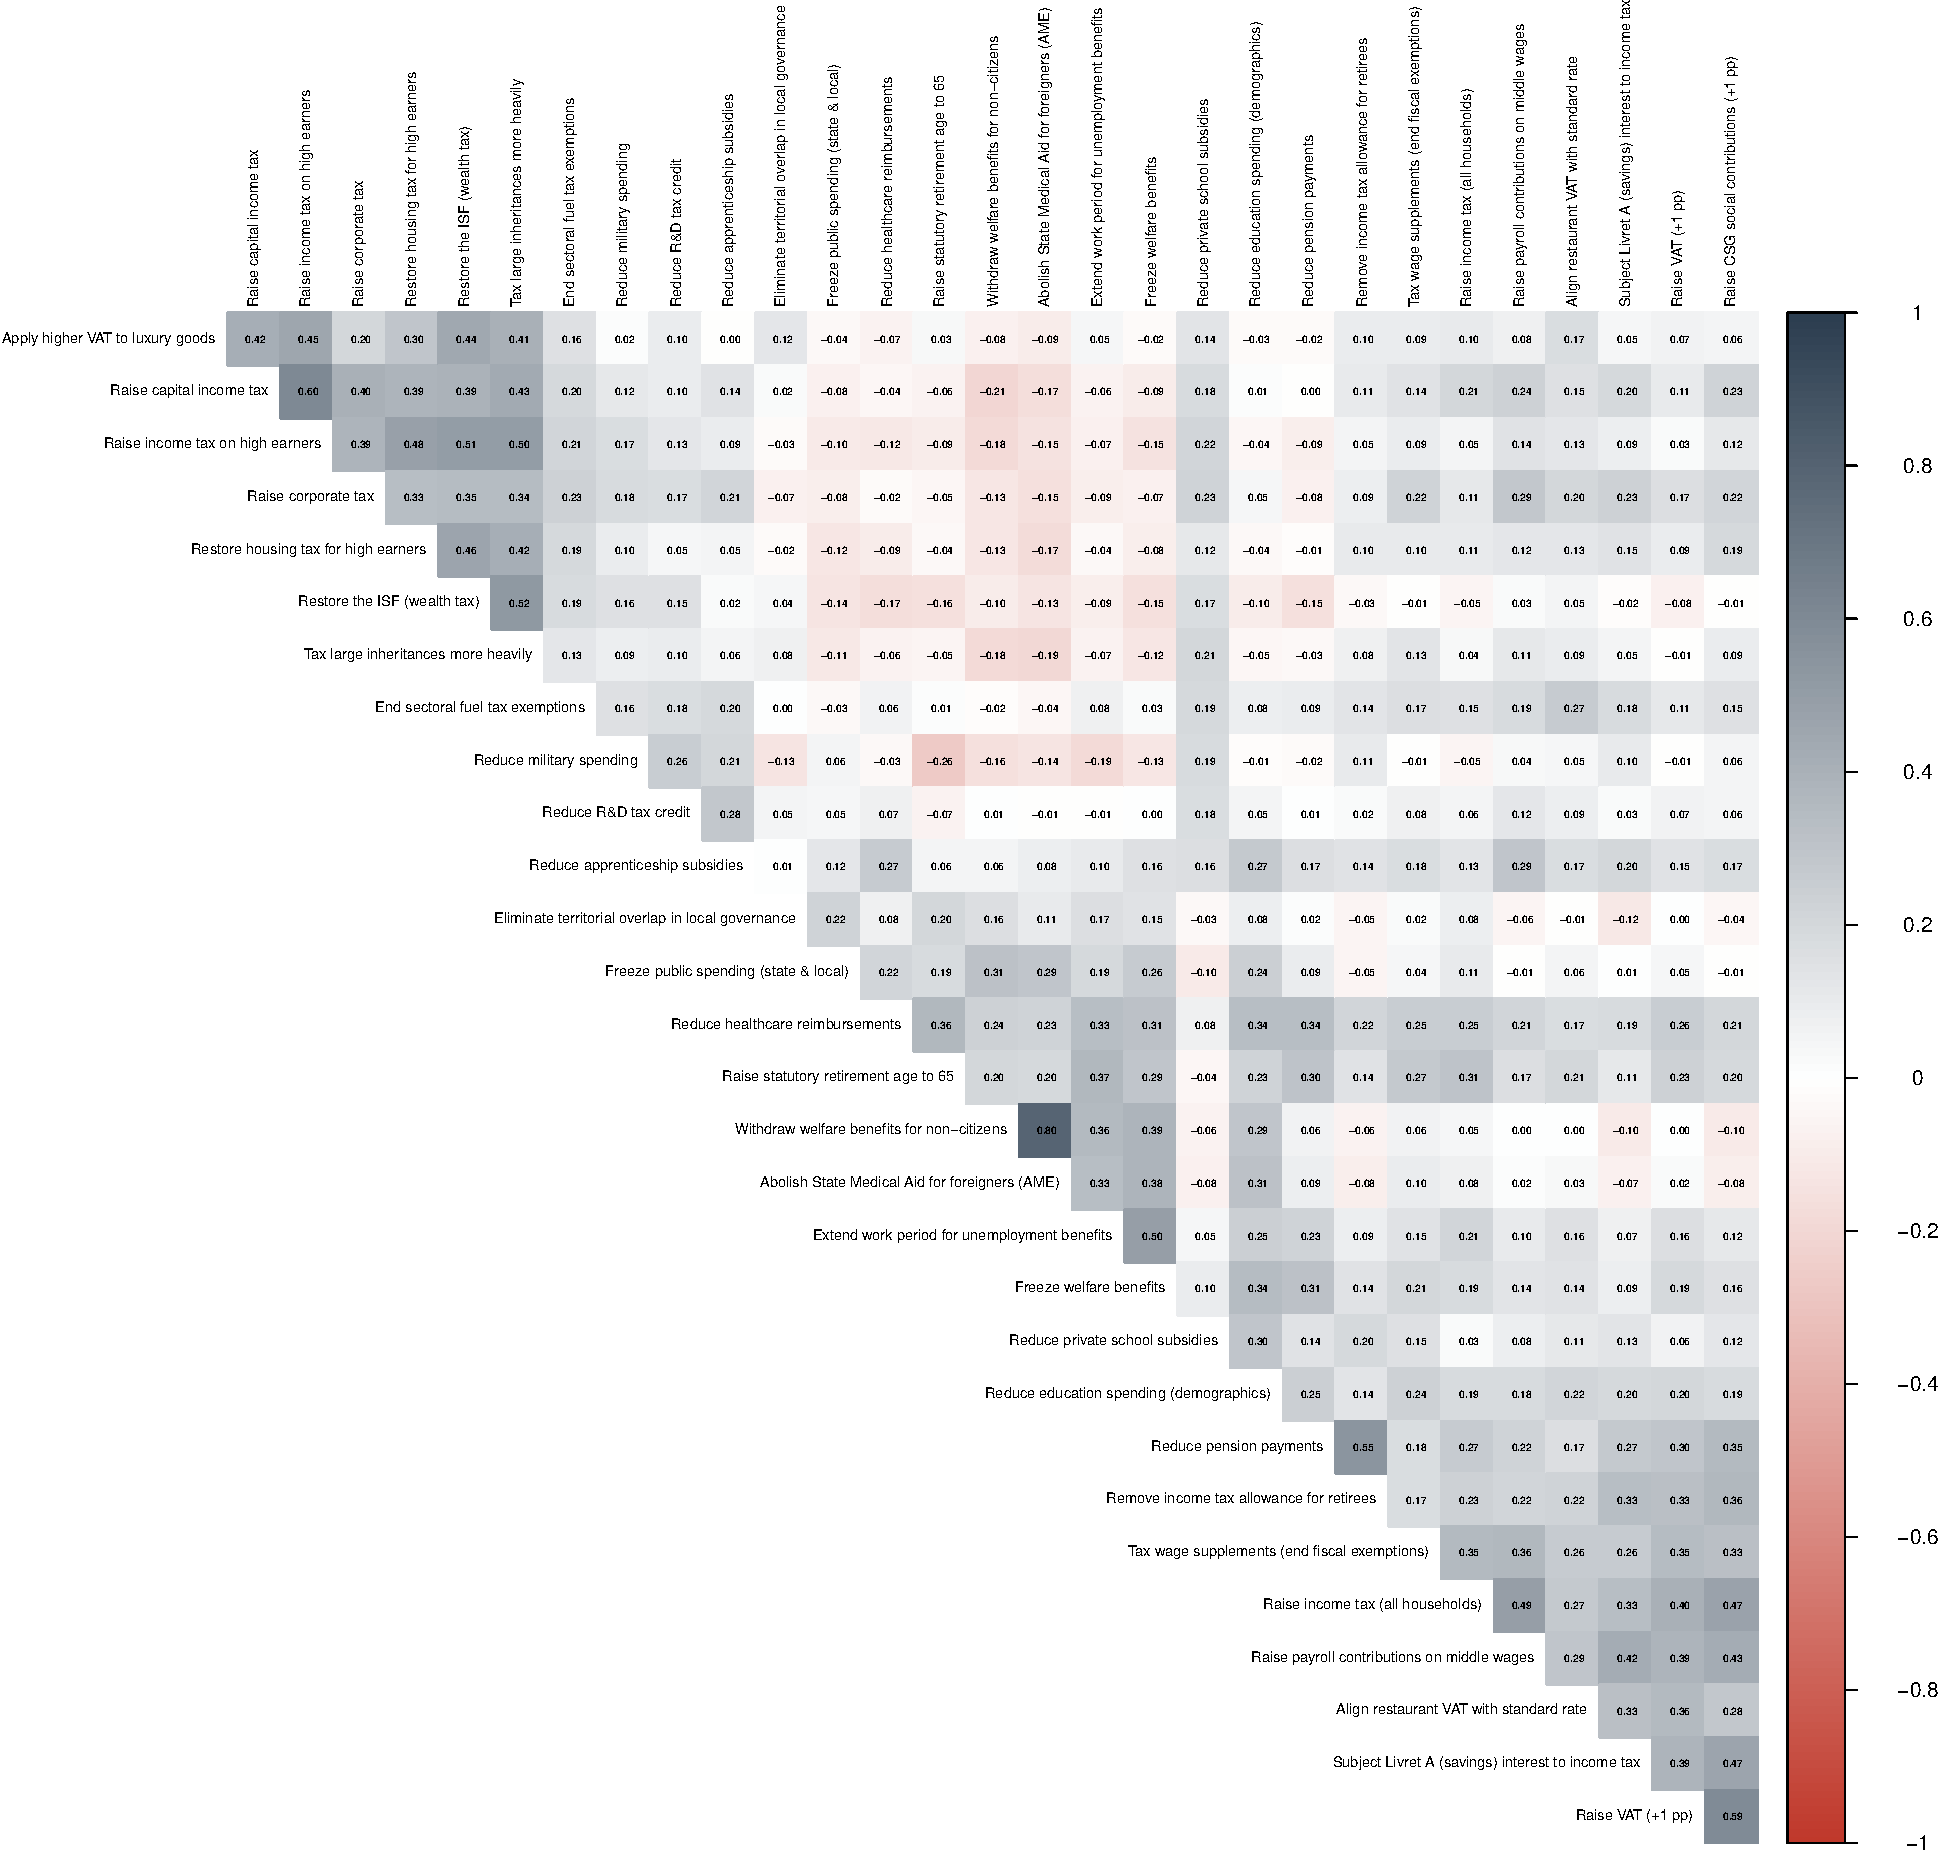
\includegraphics[width=\textwidth]{../figures/budget_correlations_en.pdf}
  \caption{Correlation matrix between assessments of fiscal measures.}
  \label{fig:budget_correlations}
\end{figure}


\begin{table}[htbp]
\centering\footnotesize\setlength{\tabcolsep}{4pt}
\noindent\makebox[\textwidth][c]{%
\begin{tabular}{lclcrccccc}
\toprule
& & & & & & \multicolumn{4}{c}{Soutien moyen (\% de convenable + souhaitable)} \\
\cmidrule(lr){7-10}
\makecell[l]{Variables\\utilisées\\(leur nombre)} & \makecell{Nombre\\de\\profils} & \makecell[l]{Description\\du profil} & \makecell{Taille\\du\\profil\\(\%)} & \makecell{Bloc\\politique\\moyen} & \makecell{Moyenne\\du paquet\\soutenu\\(Mds~€)} & \makecell{Impôt\\sur les\\riches} & \makecell{Réduit\\l'État-\\providence} & \makecell{Nativiste} & \makecell{Impôt\\indifférencié} \\
\midrule
 &  & \textbf{Ensemble} & \textbf{100} & \textbf{0\hspace{1em}} & \textbf{93} & \textbf{58} & \textbf{46} & \textbf{70} & \textbf{21} \\
\midrule
Bloc politique (1) &  & \cellcolor{cleft!15}Gauche & \cellcolor{cleft!15}28 & \cellcolor{cleft!15}$-$1\hspace{1em} & \cellcolor{cleft!15}94 & \cellcolor{cleft!15}72 & \cellcolor{cleft!15}33 & \cellcolor{cleft!15}39 & \cellcolor{cleft!15}23 \\
 &  & \cellcolor{cdjc!15}Centre-droit/Droite & \cellcolor{cdjc!15}25 & \cellcolor{cdjc!15}0\hspace{1em} & \cellcolor{cdjc!15}102 & \cellcolor{cdjc!15}52 & \cellcolor{cdjc!15}58 & \cellcolor{cdjc!15}73 & \cellcolor{cdjc!15}25 \\
 &  & \cellcolor{ced!15}Extrême-droite & \cellcolor{ced!15}30 & \cellcolor{ced!15}1\hspace{1em} & \cellcolor{ced!15}93 & \cellcolor{ced!15}51 & \cellcolor{ced!15}49 & \cellcolor{ced!15}93 & \cellcolor{ced!15}19 \\
 &  & \cellcolor{ced!15}Non-réponse/Autre & \cellcolor{ced!15}17 & \cellcolor{ced!15} & \cellcolor{ced!15}76 & \cellcolor{ced!15}58 & \cellcolor{ced!15}41 & \cellcolor{ced!15}73 & \cellcolor{ced!15}17 \\
\midrule
\texttt{budget} (30) & 2 & \cellcolor{mgt!15}Sociaux & \cellcolor{mgt!15}54 & \cellcolor{mgt!15}$-$0,3\hspace{1em} & \cellcolor{mgt!15}103 & \cellcolor{mgt!15}80 & \cellcolor{mgt!15}41 & \cellcolor{mgt!15}57 & \cellcolor{mgt!15}27 \\
 &  & \cellcolor{cdroite!15}Conservateurs & \cellcolor{cdroite!15}46 & \cellcolor{cdroite!15}0,4\hspace{1em} & \cellcolor{cdroite!15}81 & \cellcolor{cdroite!15}35 & \cellcolor{cdroite!15}51 & \cellcolor{cdroite!15}83 & \cellcolor{cdroite!15}15 \\
\midrule
{\bfseries \texttt{budget} (30)} & \textbf{3} & \cellcolor{cleft!15}Progressistes & \cellcolor{cleft!15}31 & \cellcolor{cleft!15}$-$0,5\hspace{1em} & \cellcolor{cleft!15}84 & \cellcolor{cleft!15}77 & \cellcolor{cleft!15}23 & \cellcolor{cleft!15}37 & \cellcolor{cleft!15}12 \\
 &  & \cellcolor{cfrug!15}Frugaux & \cellcolor{cfrug!15}21 & \cellcolor{cfrug!15}$-$0\hspace{1em} & \cellcolor{cfrug!15}146 & \cellcolor{cfrug!15}76 & \cellcolor{cfrug!15}70 & \cellcolor{cfrug!15}84 & \cellcolor{cfrug!15}55 \\
 &  & \cellcolor{cdroite!15}Conservateurs & \cellcolor{cdroite!15}48 & \cellcolor{cdroite!15}0,4\hspace{1em} & \cellcolor{cdroite!15}75 & \cellcolor{cdroite!15}37 & \cellcolor{cdroite!15}49 & \cellcolor{cdroite!15}86 & \cellcolor{cdroite!15}12 \\
\midrule
\texttt{budget} (30) & 4 & \cellcolor{cleft!15}Progressistes & \cellcolor{cleft!15}21 & \cellcolor{cleft!15}$-$0,8\hspace{1em} & \cellcolor{cleft!15}80 & \cellcolor{cleft!15}74 & \cellcolor{cleft!15}18 & \cellcolor{cleft!15}11 & \cellcolor{cleft!15}14 \\
 &  & \cellcolor{cfrug!15}Frugaux & \cellcolor{cfrug!15}18 & \cellcolor{cfrug!15}$-$0,1\hspace{1em} & \cellcolor{cfrug!15}150 & \cellcolor{cfrug!15}78 & \cellcolor{cfrug!15}70 & \cellcolor{cfrug!15}79 & \cellcolor{cfrug!15}59 \\
 &  & \cellcolor{ccdroit!15}Libéraux-nativistes & \cellcolor{ccdroit!15}24 & \cellcolor{ccdroit!15}0,4\hspace{1em} & \cellcolor{ccdroit!15}76 & \cellcolor{ccdroit!15}23 & \cellcolor{ccdroit!15}52 & \cellcolor{ccdroit!15}83 & \cellcolor{ccdroit!15}15 \\
 &  & \cellcolor{ced!15}Sociaux-nativistes & \cellcolor{ced!15}36 & \cellcolor{ced!15}0,4\hspace{1em} & \cellcolor{ced!15}83 & \cellcolor{ced!15}65 & \cellcolor{ced!15}45 & \cellcolor{ced!15}92 & \cellcolor{ced!15}10 \\
\midrule
{\bfseries \texttt{programme} (17)} & \textbf{2} & \cellcolor{cleft!15}Progressistes & \cellcolor{cleft!15}43 & \cellcolor{cleft!15}$-$0,5\hspace{1em} & \cellcolor{cleft!15}90 & \cellcolor{cleft!15}68 & \cellcolor{cleft!15}35 & \cellcolor{cleft!15}39 & \cellcolor{cleft!15}25 \\
 &  & \cellcolor{cdroite!15}Nativistes & \cellcolor{cdroite!15}57 & \cellcolor{cdroite!15}0,4\hspace{1em} & \cellcolor{cdroite!15}95 & \cellcolor{cdroite!15}51 & \cellcolor{cdroite!15}53 & \cellcolor{cdroite!15}91 & \cellcolor{cdroite!15}19 \\
\midrule
\texttt{programme} (17) & 3 & \cellcolor{cleft!15}Progressistes & \cellcolor{cleft!15}37 & \cellcolor{cleft!15}$-$0,5\hspace{1em} & \cellcolor{cleft!15}89 & \cellcolor{cleft!15}69 & \cellcolor{cleft!15}34 & \cellcolor{cleft!15}35 & \cellcolor{cleft!15}25 \\
 &  & \cellcolor{ccdroit!15}Libéraux-nativistes & \cellcolor{ccdroit!15}26 & \cellcolor{ccdroit!15}0,2\hspace{1em} & \cellcolor{ccdroit!15}101 & \cellcolor{ccdroit!15}45 & \cellcolor{ccdroit!15}65 & \cellcolor{ccdroit!15}89 & \cellcolor{ccdroit!15}22 \\
 &  & \cellcolor{ced!15}Sociaux-nativistes & \cellcolor{ced!15}36 & \cellcolor{ced!15}0,4\hspace{1em} & \cellcolor{ced!15}90 & \cellcolor{ced!15}58 & \cellcolor{ced!15}43 & \cellcolor{ced!15}89 & \cellcolor{ced!15}17 \\
\midrule
{\bfseries Toutes (47)} & \textbf{2} & \cellcolor{cleft!15}Progressistes & \cellcolor{cleft!15}42 & \cellcolor{cleft!15}$-$0,5\hspace{1em} & \cellcolor{cleft!15}94 & \cellcolor{cleft!15}73 & \cellcolor{cleft!15}34 & \cellcolor{cleft!15}36 & \cellcolor{cleft!15}26 \\
 &  & \cellcolor{cdroite!15}Conservateurs & \cellcolor{cdroite!15}58 & \cellcolor{cdroite!15}0,4\hspace{1em} & \cellcolor{cdroite!15}92 & \cellcolor{cdroite!15}49 & \cellcolor{cdroite!15}54 & \cellcolor{cdroite!15}93 & \cellcolor{cdroite!15}18 \\
\midrule
Toutes (47) & 3 & \cellcolor{cleft!15}Progressistes & \cellcolor{cleft!15}27 & \cellcolor{cleft!15}$-$0,7\hspace{1em} & \cellcolor{cleft!15}86 & \cellcolor{cleft!15}73 & \cellcolor{cleft!15}25 & \cellcolor{cleft!15}19 & \cellcolor{cleft!15}18 \\
 &  & \cellcolor{cdjc!15}Libéraux-frugaux & \cellcolor{cdjc!15}34 & \cellcolor{cdjc!15}0,1\hspace{1em} & \cellcolor{cdjc!15}115 & \cellcolor{cdjc!15}54 & \cellcolor{cdjc!15}71 & \cellcolor{cdjc!15}87 & \cellcolor{cdjc!15}36 \\
 &  & \cellcolor{ced!15}Sociaux-nativistes & \cellcolor{ced!15}39 & \cellcolor{ced!15}0,5\hspace{1em} & \cellcolor{ced!15}79 & \cellcolor{ced!15}52 & \cellcolor{ced!15}39 & \cellcolor{ced!15}91 & \cellcolor{ced!15}11 \\
\midrule
Toutes (47) & 4 & \cellcolor{cleft!15}Progressistes & \cellcolor{cleft!15}23 & \cellcolor{cleft!15}$-$0,8\hspace{1em} & \cellcolor{cleft!15}77 & \cellcolor{cleft!15}69 & \cellcolor{cleft!15}20 & \cellcolor{cleft!15}12 & \cellcolor{cleft!15}14 \\
 &  & \cellcolor{cfrug!15}Frugaux & \cellcolor{cfrug!15}23 & \cellcolor{cfrug!15}$-$0,1\hspace{1em} & \cellcolor{cfrug!15}128 & \cellcolor{cfrug!15}77 & \cellcolor{cfrug!15}66 & \cellcolor{cfrug!15}78 & \cellcolor{cfrug!15}51 \\
 &  & \cellcolor{ccdroit!15}Libéraux-nativistes & \cellcolor{ccdroit!15}19 & \cellcolor{ccdroit!15}0,4\hspace{1em} & \cellcolor{ccdroit!15}92 & \cellcolor{ccdroit!15}30 & \cellcolor{ccdroit!15}68 & \cellcolor{ccdroit!15}91 & \cellcolor{ccdroit!15}21 \\
 &  & \cellcolor{ced!15}Sociaux-nativistes & \cellcolor{ced!15}35 & \cellcolor{ced!15}0,5\hspace{1em} & \cellcolor{ced!15}80 & \cellcolor{ced!15}56 & \cellcolor{ced!15}37 & \cellcolor{ced!15}91 & \cellcolor{ced!15}9 \\
\bottomrule
\end{tabular}}

\caption{Respondent profiles for various clusterings (varying variables used and number of profiles) by political bloc. Profile descriptions and colors are chosen based on their characteristics. \textit{Political bloc} codes actual or hypothetical vote between $-$1 (Left) and 1 (Far right). \textit{Package supported} corresponds to the savings generated by measures rated \textit{appropriate} or \textit{desirable} by the respondent. \texttt{Budget} measures (excluding sectoral measures) are divided into four categories and the final columns report average support for measures in these categories, by profile. For each set of variables used, bold indicates the most relevant clustering (the one with the highest silhouette score, which combines cohesion and separation).}
\label{tab:cluster_comparison}
\end{table}

\begin{figure}[htbp]
  \centering
  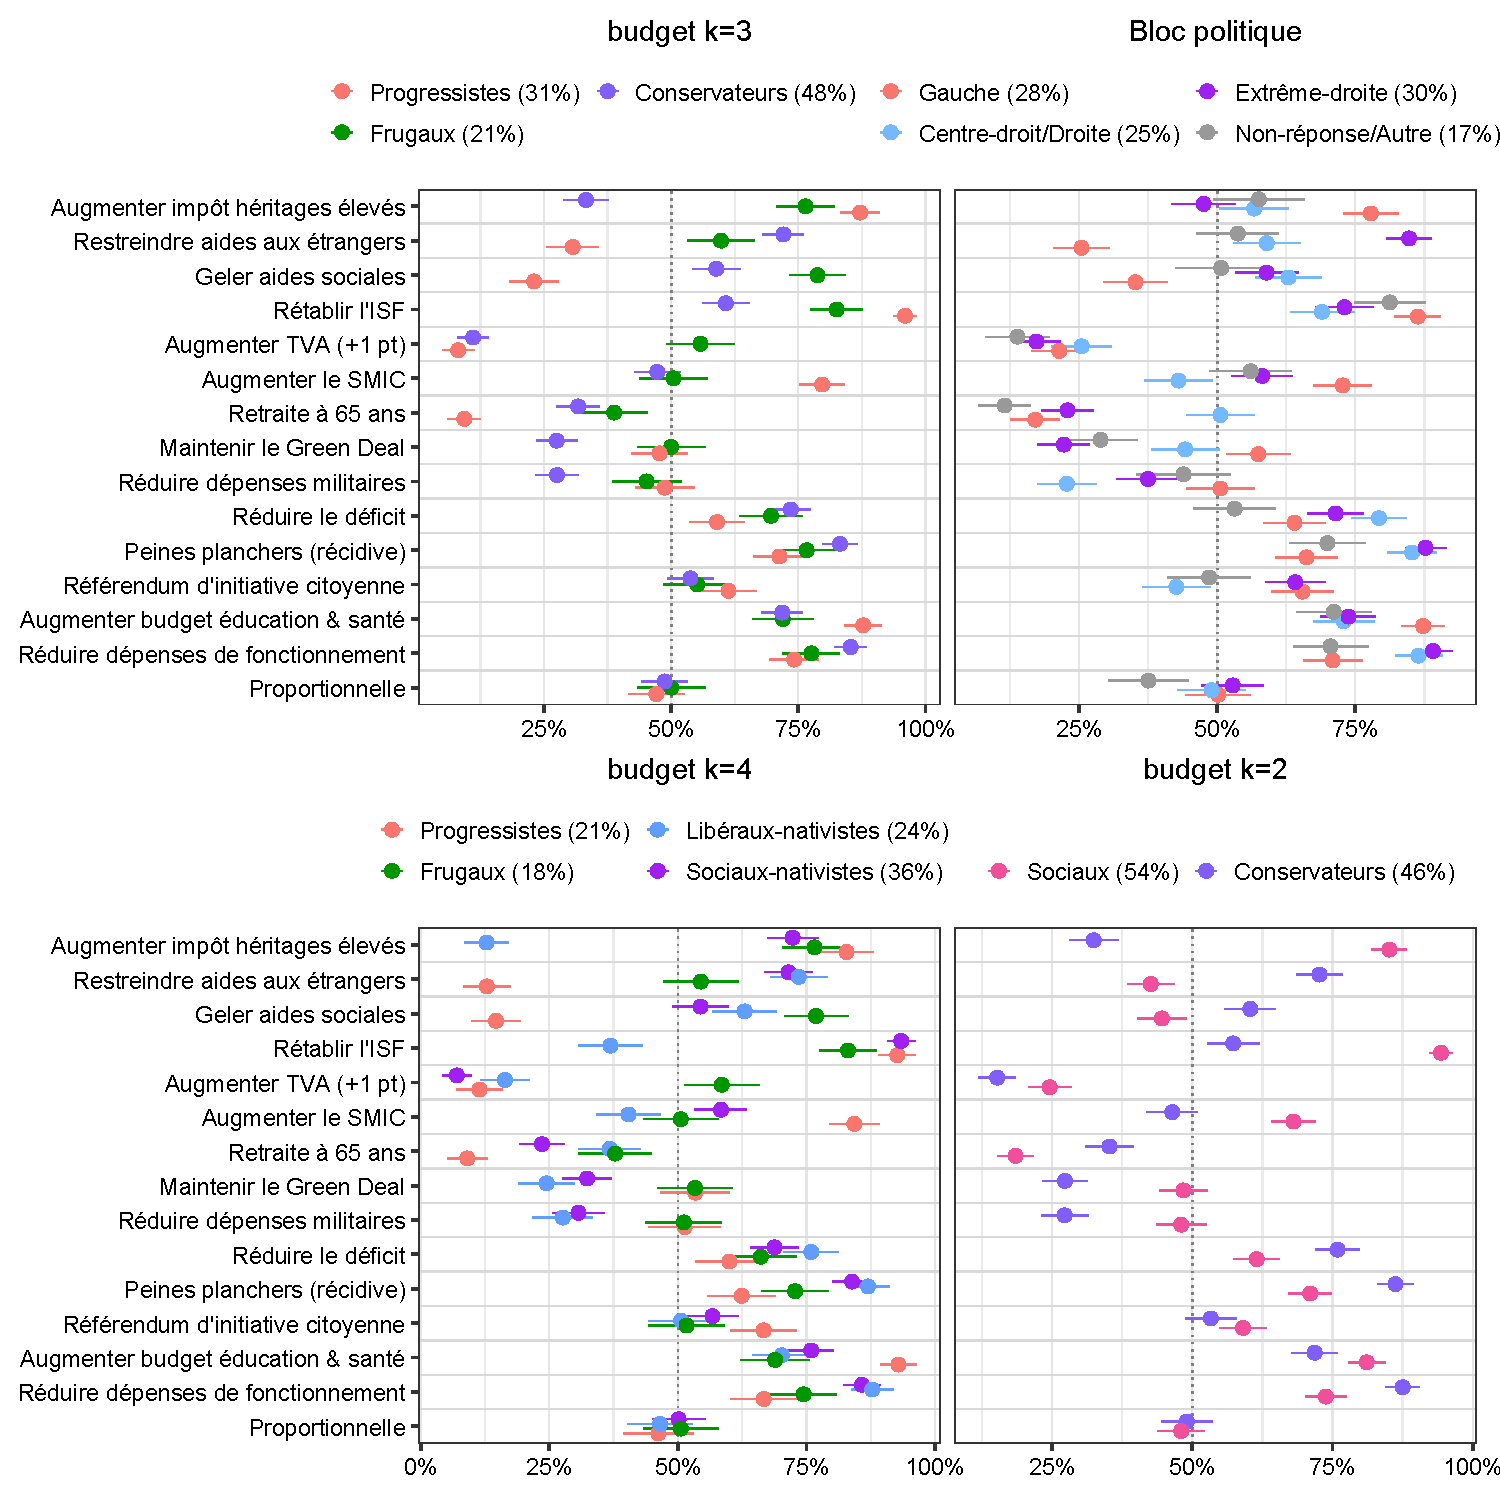
\includegraphics[width=\linewidth]{../figures/clusters_combined_polarises.pdf}
  \caption{Most polarizing attitudes by type of respondent clustering. \texttt{budget} and \texttt{programme} measures with the greatest inter-profile gap, for clustering by political bloc (top right), by \texttt{budget} profile at $k=3$ (top left) and $k=4$ (bottom left), and at $k=2$ (bottom right). Dots indicate mean support rates (\textit{appropriate} or \textit{desirable}) with 95\% confidence intervals.}
  \label{fig:clusters_combined_polarises}
\end{figure}

\end{document}
